\documentclass[12pt]{report}
\usepackage{multirow}
\usepackage{rotating}
\usepackage{hhline}
\usepackage[]{graphicx}
\usepackage[left=1.25in, right=1in,top=1in,bottom=1in,headheight=6pt, a4paper]{geometry}
\usepackage{titling}
\usepackage{booktabs}
\usepackage{natbib}
% \usepackage{biblatex}
% \usepackage{times}

\usepackage{microtype}
\usepackage[utf8x]{inputenc}
\usepackage{xcolor}
\usepackage{datetime2}

\usepackage{enumitem}
\usepackage[font=normalsize,tableposition=top]{caption}
\usepackage{etoolbox}\usepackage{setspace}
\usepackage[explicit]{}
\usepackage{algpseudocode, algorithm}
\usepackage{amsmath}
\usepackage{amsfonts}
\usepackage{amssymb}
\usepackage{hyperref}
\usepackage{pgfgantt}
\usepackage{adjustbox}
\usepackage{multicol}
\usepackage{mathptmx}
\usepackage{titlesec}
\usepackage{setspace}
\usepackage{import}
\usepackage{enumitem}
\usepackage{bm}
\usepackage{amsmath, amsfonts}
\usepackage{pdflscape}
\usepackage{everypage-1x}
\usepackage{wrapfig}
\usepackage{scrextend}
\usepackage{etoolbox}
\usepackage{appendix}
\usepackage{tabularx}
\usepackage{array}
\usepackage{listings}


\renewcommand\appendixtocname{APPENDIX}
\renewcommand\appendixpagename{APPENDIX}
\renewcommand{\bibname}{REFERENCES}

%\usetikzlibrary{positioning}
% \ganttset{group/.append style={orange},
% milestone/.append style={red},
% progress label node anchor/.append style={text=red}}

\linespread{1.3}
\setlength{\parskip}{6pt}
\setlength{\parindent}{0em}


%--------------------



%------ SET DOCUMENT GEOMETRY ------%
\usepackage{geometry}
\geometry{a4paper, left=1.25in, top=1in, bottom=1in, right=1in}


%------ FORMAT CHAPTER, SECTION, AND SUBSECTION TITLE ------%
  \titleformat{\chapter}{
  \normalfont\fontsize{16}{15}\bfseries
  }{\thechapter}{1em}{}

  \titleformat{\section}{
  \normalfont\fontsize{14}{15}\bfseries
  }{\thesection}{1em}{}

  \titleformat{\subsection}{
  \normalfont\fontsize{12}{15}\bfseries
  }{\thesubsection}{1em}{}

  \titlespacing{\chapter}{0pt}{-0.5in}{-0.5em}
  \titlespacing{\section}{0pt}{0pt}{-1em}
  \titlespacing{\subsection}{0pt}{0pt}{-1em}


%------ SET SPACING AND INDENTS ------%
\renewcommand{\baselinestretch}{1.5} 
\setlength{\parindent}{0pt}
\setlength{\parskip}{12pt}


%------ SETUP LINKS ------%
\usepackage{hyperref}
\hypersetup{
    colorlinks,
    citecolor=black,
    filecolor=black,
    linkcolor=black,
    urlcolor=black
}


%------ FORMAT TABLE OF CONTENTS ------%
\usepackage{tocloft}


\cftsetindents{section}{1.4em}{1.75em}
\cftsetindents{subsection}{3.2em}{2.6em}
\setlength{\cftbeforetoctitleskip}{-2.5em}
\setlength{\cftbeforechapskip}{0.25em}

\renewcommand{\cftchapleader}{\dotfill}

\renewcommand{\cftdotsep}{1.5}
\renewcommand{\cftsecfont}{\normalfont}
\renewcommand{\cftsecpagefont}{\normalfont}

\setlength{\cftbeforeloftitleskip}{-2.5em}
\setlength{\cftbeforelottitleskip}{-2.5em}

\setlength{\cftfigindent}{0pt}
\setlength{\cfttabindent}{0pt}

\renewcommand{\cftfigfont}{Figure }
\renewcommand{\cfttabfont}{Table }


%------ FORMAT TABLE CAPTIONS ------%
\usepackage{caption} 
\captionsetup[table]{skip=10pt}
\captionsetup[figure]{labelfont=bf,textfont=bf}
\captionsetup[table]{labelfont=bf,textfont=bf}


\newcommand{\Lpagenumber}{\ifdim\textwidth=\linewidth\else\bgroup
  \dimendef\margin=0 %use \margin instead of \dimen0
  \ifodd\value{page}\margin=\oddsidemargin
  \else\margin=\evensidemargin
  \fi
  \raisebox{\dimexpr -\topmargin-\headheight-\headsep-0.5\linewidth}[0pt][0pt]{%
    \rlap{\hspace{\dimexpr \margin+\textheight+\footskip}%
    \llap{\rotatebox{90}{\thepage}}}}%
\egroup\fi}
\AddEverypageHook{\Lpagenumber}%


\newcommand{\theinstitute}{Faculty of Humanities and Social Sciences }
\newcommand{\thecampus}{Lalitpur Engineering College }
\newcommand{\thedepartment}{Department of Computer Application }
\newcommand{\thedepartmentAddress}{Lalitpur, Nepal }
\newcommand{\thedepartmentFullAddress}{Patan, Lalitpur, Nepal }
\newcommand{\theprogramcoordinator}{Er. Bibat Thokar }
\newcommand{\theHOD}{Er.Bibat Thokar }
\newcommand{\authorWithAnd}{Sirjan Shrestha (LEC077BCA06) and Sujal Maharjan (LEC077BCA07)}


\title{BUILD WIZARD : PC PART PICKER}
\author{Sirjan Shrestha (LEC077BCA06)\\ Sujal Maharjan (LEC077BCA07) }
\newcommand{\theroll}{
  % LEC077BCA06\\LEC077BCA07
}
\date{October 2023}
\newcommand{\thesupervisor}{Er. Sandesh Sharan Poudel}


\linespread{1.5}
\begin{document}

\pagenumbering{roman}

\thispagestyle{empty}
\begin{center}
\begin{spacing}{1.6}


\includegraphics[scale=0.20]{img/Graphics/TUlogo.jpg}

\textbf{
\large{TRIBHUVAN UNIVERSITY}\\
\MakeUppercase{\large{\theinstitute}}\\
\MakeUppercase{\large{\thecampus}}}

\vspace{0.5cm}

\hspace{-8cm}
% \textbf{PROJECT NO.: \theroll}

\vspace{0.5cm}

\textbf{\MakeUppercase{\thetitle}\\
\vspace{0.5cm} 
BY \\ 
\MakeUppercase{\theauthor}}

\vspace{0.5cm}

\textbf{  A PROJECT\\
SUBMITTED TO THE \MakeUppercase{\thedepartment}\\ IN PARTIAL FULFILLMENT OF THE REQUIREMENT FOR\\ THE DEGREE OF BACHELORS IN COMPUTER APPLICATION}
\bigskip

\par
\textbf{\MakeUppercase{\thedepartment}}\\
\textbf{\MakeUppercase{\thedepartmentAddress}}
\vspace{1cm}

\textbf{\MakeUppercase{October 2023}}



\end{spacing}
\end{center}

\clearpage
\begin{center}
\begin{spacing}{1.6}
\thispagestyle{empty}


\includegraphics[scale=0.20]{img/Graphics/TUlogo.jpg}

\textbf{
\large{Tribhuvan University}\\
\large{\theinstitute}}\\
\vspace{0.5cm}
\textbf{\MakeUppercase{\thetitle}\\
\vspace{0.5cm} 
Submitted to\\ 
\thedepartment\\
\thecampus}\\
\vspace{0.5cm}

\textbf{In partial fulfillment of the requirement for the degree of Bachelors in Computer Application}
\bigskip

\par

\textbf{
Submitted by\\
\theauthor\\
\MakeUppercase{\thedate}}\\
\vspace{1cm}
\textbf{
Under the Supervision of\\
\thesupervisor
}
\end{spacing}
\end{center}

\clearpage
%\chapter*{\centerline{COPYRIGHT \textcopyright}}
\addcontentsline{toc}{chapter}{COPYRIGHT}
\vspace{-0.5cm}

The author has agreed that the library, \thedepartment, \theinstitute, \thecampus, may make this project
work freely available for inspection. Moreover the author has agreed that the
permission for extensive copying of this project work for scholarly purpose may be
granted by the professor(s), who supervised the project work recorded herein or, in
their absence, by the Head of the Department, wherein this project work was done. It
is understood that the recognition will be given to the author of this project work and
to the \thedepartment, \theinstitute, \thecampus \ in any use of the material of this project work. Copying of publication or other use of
this project work for financial gain without approval of the \thedepartment, \theinstitute, \thecampus \ and author’s
written permission is prohibited.

Request for permission to copy or to make any use of the material in this thesis in
whole or part should be addressed to:

\vspace{1cm}

Head\\
\thedepartment\\
\theinstitute, \thecampus\\
\thedepartmentFullAddress

\chapter*{\centerline{DECLARATION}}
\addcontentsline{toc}{chapter}{DECLARATION}
\vspace{-0.5cm}
I declare that the work hereby submitted for Bachelors in Computer Application at the \thedepartment, \thecampus \ entitled "\textbf{\thetitle}" is my own work and has not been previously submitted by
me at any university for any academic award.
I authorize the \thedepartment, \thecampus \ to lend this project work
to other institutions or individuals for the purpose of scholarly research.

\vspace{1cm}

\textbf{\theauthor} \\
\theroll \\
\thedate
\newgeometry{left=1.5in, top=2.5in, bottom=1in, right=1in}
\chapter*{\centerline{RECOMMENDATION}}
\addcontentsline{toc}{chapter}{RECOMMENDATION}
\vspace{-0.5cm}
The undersigned certify that they have read and recommend to the \thedepartment \ for acceptance, a project work entitled “\textbf{\thetitle}”, submitted by \textbf{\authorWithAnd} in partial fulfillment of the requirement
for the award of the degree of “\textbf{Bachelors in Computer Application}”.

\vspace{1cm}
\rule{0.5\textwidth}{0.4pt}\\
\textbf{Project Supervisor}\\
\thesupervisor\\
Lecturer\\
\thedepartment, Lalitpur Engineering College\\

\vspace{1cm}
\rule{0.5\textwidth}{0.4pt}\\
\textbf{BCA Program Coordinator}\\
\theprogramcoordinator\\
Lecturer\\
\thedepartment, \thecampus\\

\vspace{1cm}
\thedate
\restoregeometry
\newgeometry{left=1.5in, top=2.5in, bottom=1in, right=1in}
\chapter*{\centerline{DEPARTMENTAL ACCEPTANCE}}
\addcontentsline{toc}{chapter}{DEPARTMENTAL ACCEPTANCE}
\vspace{-0.5cm}
The project work entitled “\textbf{\thetitle}”, submitted by \textbf {\authorWithAnd }in
partial fulfillment of the requirement for the award of the degree of “\textbf{Bachelors of Computer Application}” has been accepted as
a genuine record of work independently carried out by the student in the department.

\vspace{5cm}

\begin{addmargin}[5.5cm]{0em}
\rule{0.62\textwidth}{0.4pt}\\
\textbf{\theHOD}\\
BCA Coordinator\\
\thedepartment,\\
\thecampus,\\
\theinstitute,\\
Tribhuvan University,
Nepal.\\
\end{addmargin}

\vspace{2cm}

\thedate

\restoregeometry
\newcolumntype{Y}{>{\centering\arraybackslash}X}


\begin{figure}
    \centering
    
\includegraphics[width=1.8in]{img/Graphics/TUlogo.jpg
    }
\end{figure}

\begin{center}
    {\fontsize{14pt}{18}\selectfont
    \textbf{Tribhuvan University\\
    Faculty of Humanities and Social Sciences\\
    Lalitpur Engineering College\\
    \vspace{0.2in}
    LETTER OF APPROVAL\\}
    \vspace{0.2in}}
\end{center}

This is to certify that this project prepared by Sujal Maharjan and Sirjan Shrestha entitled “\textbf{Build Wizard:Pc Part Picker}” in partial fulfillment of the requirements for the degree of Bachelor in Computer Application has been evaluated. In our opinion, it is satisfactory in the scope and quality as a project for the required degree.
\begin{center}
    {\fontsize{14pt}{18}\selectfont
    \begin{table}[ht]
        \begin{tabularx}{\textwidth}{|Y|Y|}
        \hline
        &\\
        &\\
        ..............................................................&..............................................................\\
        &\\
        Er. Sandesh Sharan Poudel & Er. Bibat Thokar \\
        Project Supervisor & BCA Program Coordinator \\
        Department of Computer Application & Department of Computer Application\\
        Lalitpur Engineering College & Lalitpur Engineering College \\
        &\\
        &\\
        \hline
        &\\
        &\\
        .............................................................. & ..............................................................\\
        &\\
        Er. Praches Acharya & Prof. Dr. Subarna Shakya\\
        Internal Examiner&External Examiner\\
        Head of Department & Professor, Subject Committee Member\\
        Department of Computer Engineering & Institute of Engineering \\
        Lalitpur Engineering College & Pulchowk Campus \\
        \hline
        \end{tabularx}
        \end{table}
    }
\end{center}
\chapter*{\centerline{ACKNOWLEDGMENT}}
\addcontentsline{toc}{chapter}{ACKNOWLEDGMENT}
\vspace{-0.5cm}
This project work would not have been possible without the guidance and the help of
several individuals who in one way or another contributed and extended their
valuable assistance in the preparation and completion of this study.


First of all, I would like to express my sincere gratitude to my supervisor, \textbf{\thesupervisor}, of \textbf{\thecampus} for providing invaluable guidance, insightful comments, meticulous suggestions, and encouragement throughout the duration of
this project work. My sincere thanks also goes to the BCA coordinator, \textbf{\theprogramcoordinator}, for coordinating the project works, providing astute criticism, and having
inexhaustible patience.

Furthermore, we would like to extend our gratitude to the entire faculty of the \thedepartment. Their dedication to fostering creativity, critical thinking, and technical proficiency has been useful in our project's development. The support and guidance received from our teachers have empowered us to transform our vision into a reality.

I am also grateful to my classmates and friends for offering me advice and moral
support. To my family, thank you for encouraging me in all of my pursuits and
inspiring me to follow my dreams. I am especially grateful to my parents, who
supported me emotionally, believed in me and wanted the best for me.

\vspace{1cm}

\textbf{\theauthor} \\
\theroll \\
\thedate

%==============================Abstract Page=================================================
\chapter*{\centerline{ABSTRACT}}
\addcontentsline{toc}{chapter}{ABSTRACT}
\thispagestyle{plain} 
% Abstract (200 to 250 Words)
\vspace{-0.5cm}

Build Wizard is a web-based platform designed to simplify the process of selecting compatible components for custom PC builds. It provides a comprehensive database of PC components, including processors, motherboards, graphics cards, memory modules, storage drives, power supplies, and more.
The platform offers an intuitive user interface that allows  enthusiasts, and professionals to create, customize, and compare PC builds tailored to their specific requirements. Users can search for components based on various criteria such as brand, performance, price, and compatibility. Build Wizard ensures that selected components are compatible with each other, preventing common pitfalls that arise from incompatible hardware combinations.
In addition to component selection, Build Wizard also provides up-to-date pricing information from various retailers, enabling users to make informed decisions based on budget constraints. The platform assists in comparing prices across different vendors, ensuring users can find the best deals for their chosen components.\\\\
\textbf{Keywords:}  \textit{Compare price}, \textit{Compatible components}, \textit{Customize}
%=============================================================================================
% (a) Inclusion of three to four Keywords (Lexicographical Order)
% \newpage
% \chapter*{\centerline{AKNOWLEDGEMENT}}
% We would like to extend our heartfelt gratitude to the esteemed teachers in the \thedepartment at \thecampus for their invaluable support and guidance throughout the development of our social network application.

% First and foremost, we would like to express our deepest appreciation to \thesupervisor and \theprogramcoordinator, both our project supervisor and program coordinator, for their unwavering commitment,mentorship to our project. Their expertise and profound knowledge in this field have been very helpful in shaping our technical skills and providing invaluable insights of the projects.

% Furthermore, we would like to extend our gratitude to the entire faculty of the \thedepartment. Their dedication to fostering creativity, critical thinking, and technical proficiency has been useful in our project's development. The support and guidance received from our teachers have empowered us to transform our vision into a reality.

% Your unwavering belief in our abilities and your constant encouragement have been the driving force behind our project. Your passion for education and commitment to our growth have left an indelible impact on our personal and professional development.


% Sincerely,\\
% \theauthor\\
% \thedepartment\\
% \thecampus\\
\newpage

%=================TOC=========================================================================

\cftsetindents{section}{1.5em}{2.1em}
\cftsetindents{subsection}{3.6em}{3.1em}

\chapter*{\centerline{TABLE OF CONTENTS}}
\addcontentsline{toc}{chapter}{TABLE OF CONTENTS}
\def\contentsname{\empty}
\tableofcontents
\clearpage




\chapter*{\centerline{LIST OF FIGURES}}
\addcontentsline{toc}{chapter}{LIST OF FIGURES}
\def\listfigurename{\empty}
\newcommand*{\noaddvspace}{\renewcommand*{\addvspace}[1]{}}
\addtocontents{lof}{\protect\noaddvspace}
\listoffigures
\clearpage


\chapter*{\centerline{LIST OF TABLES}}
\addcontentsline{toc}{chapter}{LIST OF TABLES}
\def\listtablename{\empty}
\addtocontents{lot}{\protect\noaddvspace}
\listoftables
\clearpage




%================Abbreviation Page=====================================
\chapter*{\centerline{LIST OF ABBREVIATIONS}}
\addcontentsline{toc}{chapter}{LIST OF ABBREVIATIONS}

% ABBR\hspace:   ABBREVIATIONS\\



\begin{tabular}{l@{\hspace{3cm}}p{15cm}}
 
  CSS & Cascading Style Sheets \\
  DFD & Data Flow Diagram \\
  DOM & Document Object Model \\
  ER & Entity-Relationship \\
  HTML & Hypertext Markup Language \\
  IT & Information Technology \\
  JS & JavaScript \\
  MySQL & My Structured Query Language \\
  OS & Operating System \\
  PHP & Hypertext Preprocessor \\
  SQL & Structured Query Language \\
  UI & User Interface \\
  URL & Uniform Resource Locator \\
  UX & User Experience \\

\end{tabular}

%===============================================================================



% \newpage
%=============================================================================


\pagenumbering{arabic}

%=====================Report Body=============================================


\chapter{INTRODUCTION}
% (20% of Proposal Length)
\pagenumbering{arabic}

% Introduction: (20\% of Report Length)


\section{Introduction}
The Build Wizard project aims to develop an innovative online platform that assists PC builders in Nepal in selecting compatible components, comparing prices, and engaging with a vibrant community. This  provides a comprehensive background for the project, outlining the need, objectives, and potential impact.The PC building industry in Nepal has witnessed significant growth in recent years, fueled by increasing demand for custom-built PCs. However, PC builders often face challenges in selecting compatible components and comparing prices across multiple retailers. The absence of a localized platform catering specifically to the Nepalese market creates a gap that the Build Wizard project intends to address.
\section{Problem Statement}

The process of selecting and assembling compatible components for custom PC builds poses significant challenges for individuals in the rapidly evolving PC building industry. With a plethora of PC components available and constant technological advancements, users face difficulties in navigating the complex landscape, often resulting in compatibility issues, time-consuming troubleshooting, and suboptimal hardware choices.\\\\
Thus,a comprehensive solution is required to address these problems, providing a user-friendly interface, an extensive and up-to-date component database, real-time pricing information, compatibility verification, and a vibrant community for sharing expertise and support. By tackling these challenges, users will be empowered to confidently select and assemble compatible PC components, optimize their budget, and create high-performance custom PC builds tailored to their specific needs and preferences
\section{Objectives}
\begin{itemize}
    \item The objective of the project is to create a comprehensive and localized solution that simplifies the PC building process.
\end{itemize}
\section{Scope}
% Scope and limitation

The scope of the Build Wizard project in Nepal would encompass providing a localized version of the platform tailored to the needs and preferences of Nepalese users. The project would aim to address the specific challenges faced by PC builders in Nepal and offer a comprehensive solution for component selection, compatibility verification and pricing comparison.\\Localized Component Database: The project would involve compiling a comprehensive and up-to-date database of PC components available in the Nepalese market. This would include processors, motherboards, graphics cards, memory modules, storage drives, power supplies, cooling solutions, peripherals, and other relevant hardware.\\
Pricing Integration: The platform would integrate with local retailers and online marketplaces to provide real-time pricing information from Nepalese vendors. This functionality would enable users to compare prices, find the best deals, and optimize their budget while making informed purchasing decisions.\\Vendor Partnerships: Collaborating with local PC component retailers and manufacturers would be crucial to ensure accurate and up-to-date information, pricing integration, and availability of components. Building partnerships with these entities would enhance the platform's credibility and provide users with a seamless experience.\\Education and Resource Hub: The platform could also feature educational content, tutorials, and resources specific to the Nepalese context, empowering users with the necessary knowledge and skills for successful PC builds.
\section{Limitation}
\begin{itemize}
    \item This system doesn't have offline customizing.
    \item The platform may not fully cater to users with limited technical expertise.
    \item Any inaccuracies or outdated data could impact compatibility checks or pricing information
 \end{itemize}
\section{Potential Applications}
 A PC part picker project has several potential applications that can benefit both individual users and the broader computing community. Some of these applications include:
\begin{itemize}
    \item Custom PC Building: The primary application is assisting users in selecting compatible components for building their own custom PCs. It streamlines the process, ensuring that the selected components work well together, and helps users optimize performance according to their needs. 
    \item Gaming Enthusiasts: Gamers often require high-performance systems. This project can aid them in building gaming rigs that meet their specific requirements, taking into account factors like graphics card capabilities, cooling solutions, and more.
    \item Educational Use: The platform can serve as an educational tool, helping students learn about different PC components, their specifications, and how they work together. It could be integrated into technology courses or workshops.
    \item DIY PC Building Workshops: Institutions or organizations offering DIY PC building workshops can utilize this tool to simplify the process for participants.
\end{itemize}
\section{Originality of Project}
The originality of a PC part picker project lies in how it innovatively addresses challenges and provides value that sets it apart from existing solutions.
\begin{itemize}
    \item Unique Feature Set: This project offers novel features not commonly found in other PC part pickers, such as advanced compatibility algorithms.
    \item Educational Aspect: This project not only helps users select components but also educates them about the technology behind each component, it can be unique in promoting learning alongside building.
\end{itemize}
\section{Report Organisation}
The material in this project report is organised into seven chapters. After this introductory chapter introduces the problem topic this research tries to address, chapter 2 contains the literature review of vital and relevant publications, pointing toward a notable research gap. Chapter 3 describes the methodology for the implementation of this project. Chapter 4 provides an overview of what has been accomplished. Chapter 5 contains some crucial discussions on the used model and methods. Chapter 6 mentions pathways for future research direction for the same problem or in the same domain. Chapter 7 concludes the project shortly, mentioning the accomplishment and comparing it with the main objectives.
\chapter{BACKGROUND AND LITERATURE REVIEW}

% (20\% of Report Length)

% a. Must be paraphrased without plagiarizing

% b. Must include the base papers\cite{Adhikari2020Dec}, and support the rationale of the project

% c. Must highlight the strengths and shortcomings of the works performed by other authors

\section{Background Study}
In today's rapidly evolving PC hardware market, the complexity of selecting and configuring PC components has surged. Users often face challenges in identifying compatible parts and optimizing their configurations. The proposed project seeks to address this issue by leveraging Bootstrap, a powerful front-end web framework, to develop an intuitive and user-friendly online platform. The objective is to simplify the process of building PC configurations by offering a structured interface, real-time updates, and seamless compatibility checks, ultimately empowering users to create their ideal PC setups efficiently.\\
By leveraging the power of Build Wizard, users can confidently navigate the vast array of PC components, unleash their creativity, and embark on the journey of building their dream computer systems.

\section{Literature Review}
The field of computer science and technology has advanced rapidly over the years, leading to significant developments in the design and assembly of personal computers (PCs). One crucial aspect of building a PC is selecting the right components, such as processors, graphics cards, memory modules, and storage devices.\\
In this research paper, the authors present PC Builder Hero, a virtual reality (VR) game that allows users to experience the process of building a custom personal computer (PC) in a safe and immersive environment. The primary objective of the game is to increase awareness and curiosity about the inner components and workings of computers. By utilizing VR technology, the game aims to provide users with a hands-on experience of building a PC, without the risk of costly mistakes. Users are able to select virtual computer components and track the price of their built computer, as well as monitor the accumulation of static electricity over time. The game challenges users to find a balance between component specifications and overall price, while adhering to proper PC building procedures. The paper provides detailed information on the design and implementation of a high-fidelity prototype of the game, along with the results and implications of an informal early testing phase\cite{slovikosky2019pc}.
The objective of this project is to assist users in buying or upgrading custom-branded PCs by providing recent information about computer components and automatically filtering for compatibility. The implementation involves web scraping for component information, building a database to store the data, and creating a user-friendly web page for component display and compatibility checks. The database is updated daily to ensure up-to-date information. The main contribution of this project is the automatic detection of component compatibility, which is particularly helpful for first-time buyers who may be hesitant to build their own PC\cite{romero2021implementing}.
A custom-built PC is assembled to cater to specific user needs. Internationally, there are many e-stores available for users that offer them the option to build and order their systems according to their requirements. However, the COVID-19 pandemic in 2020 led to cancellations of international shipments, highlighting the local market's deficiency in fulfilling the demands of custom-built PC users. In this paper, a generic architecture for an e-store called Nice PC Maker (NPM) is proposed and designed to address this issue. The architecture facilitates users with custom-build PC options, as well as additional features like pre-built system purchasing and PC component purchasing. The implementation of the architectural design utilizes WooCommerce product builders in WordPress. The configuration of this generic architecture for a local client not only helps them enhance their business but also provides users with the convenience of obtaining their desired systems\cite{khursheed2023nice}.
\chapter{SYSTEM ANALYSIS AND DESIGN}
\section{methodology}
To build a Build Wizard website in Nepal,an agile methodology with an iterative approach would be well-suited.Here's a breakdown of the methodology:
\begin{itemize}
   \item \textbf{Flexibility:}Agile is a flexible approach to project management and development.
   \item \textbf{Customer-Centric:}t prioritizes customer satisfaction and regular customer feedback.
   \item \textbf{Iterative Development:}Projects are divided into small, iterative steps for incremental progress.
   \item \textbf{Collaboration:}Cross-functional teams work closely together, promoting collaboration.
   \item \textbf{Continuous Feedback:}regular feedback loops are essential for improvement.
\end{itemize}

\section{System Analysis}
   \begin{itemize}  
      \item \textbf{Define Requirements and Scope:}
      Gather requirements  considering their needs and preferences.Clearly define the scope of the project, identifying the key features and functionalities.
      \item \textbf{Plan and Design:}
      Create prototypes to visualize the user interface.Plan the overall architecture, database structure, and technology stack for the website.
      \item \textbf{Develop Minimum Viable Product:}
      Start by building the core functionalities required for the Build Wizard, such as component search, filtering, and basic compatibility checks.
      Release an initial version of the website with the essential features to gather user feedback and validate the concept.
      
      \item \textbf{Gather User Feedback:}
      Encourage users to provide feedback on their experience, including usability, features, and any issues they encounter.
      Conduct surveys or user interviews to gain insights into user preferences, and improvements.
      
      \item \textbf{Iterative Development:}
      Based on user feedback, prioritize and implement enhancements and additional features in iterative cycles.
      Continuously refine the user interface, performance, and usability to optimize the website.
      
      \item \textbf{Test and Quality Assurance:}
      Conduct thorough testing to ensure the functionality and compatibility of the website across different devices, browsers, and operating systems.
      Identify and address any bugs, errors, or inconsistencies to improve the website's stability and reliability.
      \item \textbf{Release and Deployment:}
      Deploy the website to a production environment, ensuring proper setup and security measures.Monitor the performance of the website and address any issues that arise after the launch.
      
      \item \textbf{Continuous Improvement:}
      Regularly gather user feedback and track website analytics.
      Plan and implement updates, new features,pricing and component database expansions to keep the website relevant and up to date.
   \end{itemize}
\section{Requirement Analysis}
\subsection{functional Requirements}
\begin{itemize}
   \item \textbf{User Registration:}Users should be able to create accounts and authenticate themselves securely to access personalized features and configurations.
   \item \textbf{PC Component Selection:}Users should be able to browse and select PC components (e.g., CPU, GPU, RAM) from a categorized list.
   \item \textbf{Configuration Building:}Users should be able to add selected components to a configuration list and customize quantities based on their requirements.
   \item \textbf{Real-time Data Updates:}Prices, availability, and specifications of components should be updated in real time from reliable sources.
   \item \textbf{Admin Dashboard:}Admins should have access to a dashboard to manage users, components, reviews, and configurations.
\end{itemize}
\subsection{Non-functional Requirements}
\begin{itemize}
   \item \textbf{Performance:}The system should respond to user interactions within appropriate time to provide a seamless user experience.
   \item \textbf{User Experience and Design:}The user interface should be intuitive, visually appealing, and responsive across various devices and screen sizes.
   The design should follow usability principles, making the platform easy to navigate and understand for users.
\end{itemize}
   \section{Feasibility Analysis}
   The feasibility analysis conducted for the BuildWizard project has shed light on crucial aspects integral to its successful development, deployment, and sustainability. Key findings from each dimension of the analysis are summarized below:
   \begin{itemize}
      \item \textbf{Technical Feasibility:}The technical aspects required for the BuildWizard project, encompassing hardware, software, and technical expertise, are feasible and attainable within the proposed scope.
      \item \textbf{Schedule Feasibility:}A well-structured project timeline has been devised, accounting for necessary phases and potential time constraints to ensure timely completion.
      \item \textbf{Operational Feasibility:}The integration of BuildWizard with existing systems and workflows is feasible, and user acceptance testing will further optimize its operational efficiency.
   \end{itemize}
   \newpage
      \section{ER diagram}
      An Entity-Relationship (ER) diagram is a graphical representation used in database design to illustrate the logical structure and relationships of entities, attributes, and the associations between them within a database system. It serves as a visual tool for modeling and communicating how different components in a database are connected.\\\\
      Figure 3.2 is ER diagram of system it shows the entites of system with their attributes and relationships.
      \begin{figure}[ht]
      \centering
      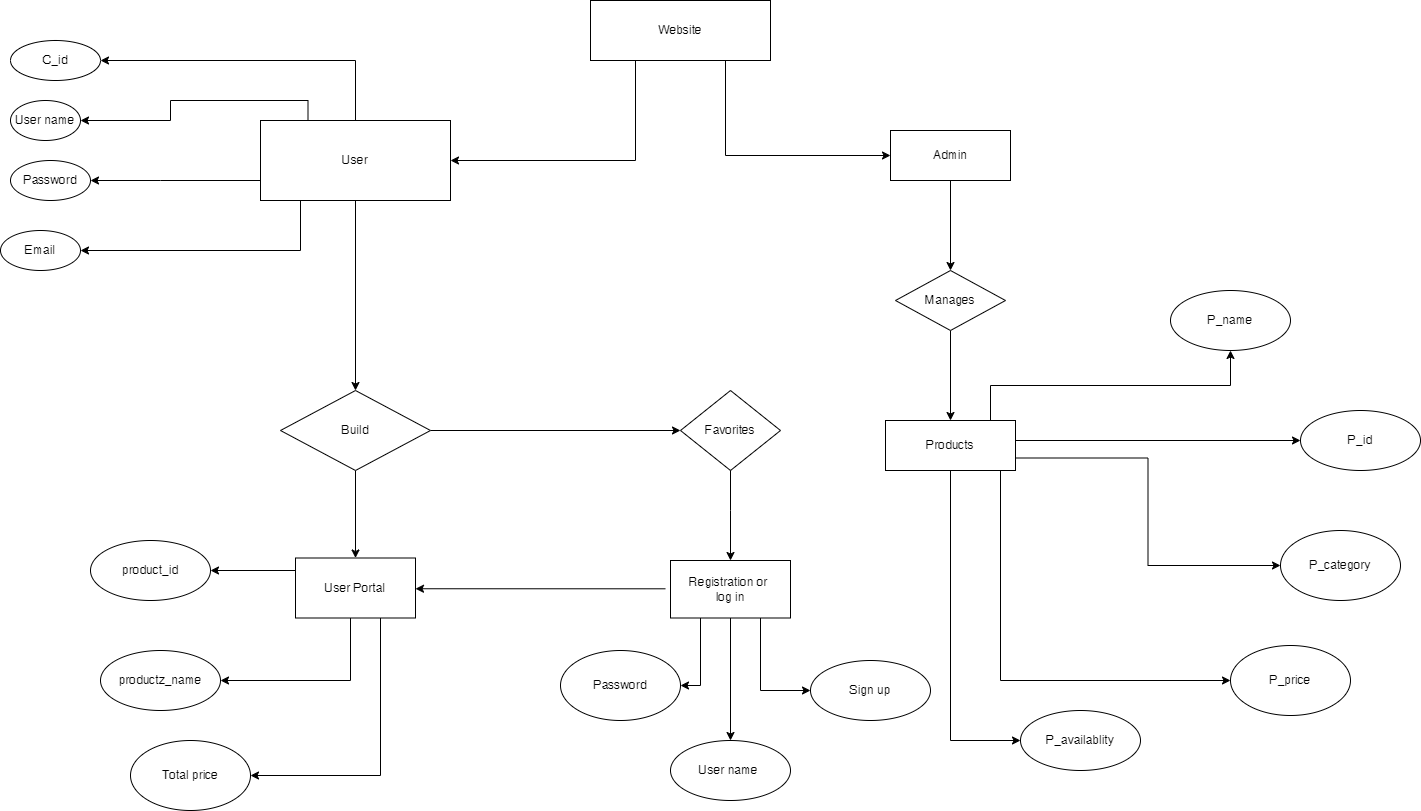
\includegraphics[width=15cm]{Diagrams/Pc_part_er_diagram.drawio.png}
      \caption{ER diagram}
      \end{figure}
      \subsection{Process Modeling(DFD)}
     \begin{figure}[ht]
      \centering
      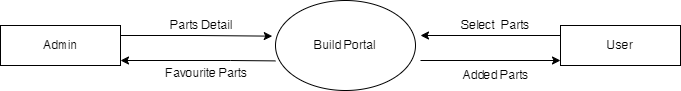
\includegraphics[width=15cm]{Diagrams/0levDFD.drawio.png}
      \caption{DFD diagram}
     \end{figure}
     \newpage
      \section{System Design}
   \subsection{Architecture design}
   Following figure shows the architecture design of this system.It shows what are the functions can be accesses after opening our site.
   \begin{figure}[H]
   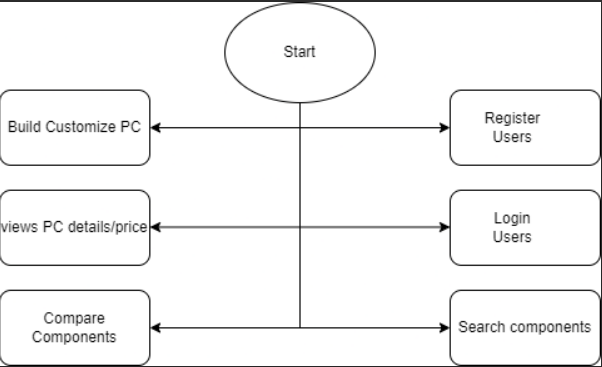
\includegraphics[width=15cm]{Diagrams/arcdesign.png}
   \caption{Architecture design}
   \end{figure}
   \newpage
   \subsection{Database Schema Design}
   Schema design, also known as database design or data modeling, is the process of structuring and organizing the data and relationships within a database system. It involves defining the tables, fields, data types, constraints, and relationships that will be used to store and manage information in a database.\\\\
   \begin{figure}[H]
   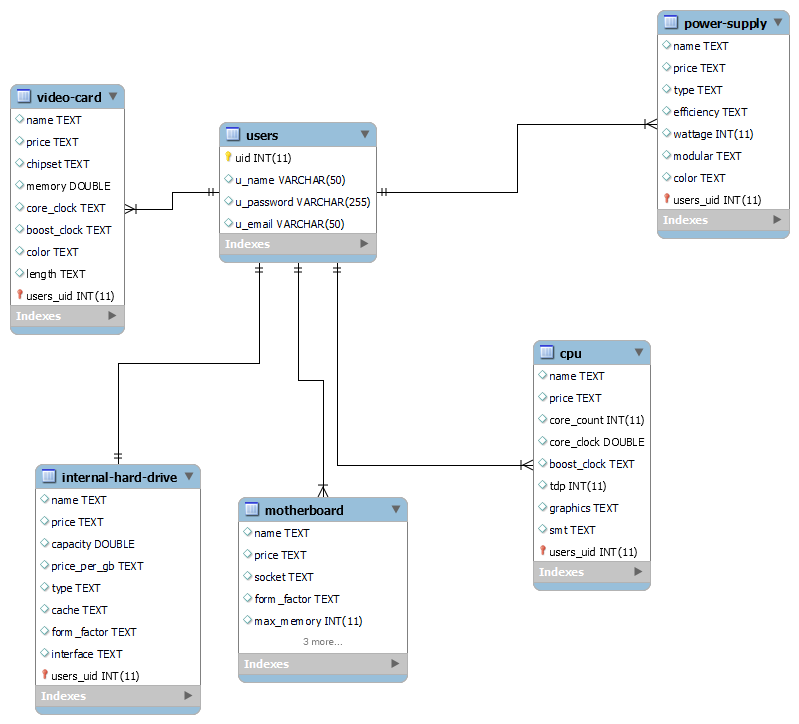
\includegraphics[width=15cm]{Diagrams/schema.png}
   \caption{Database Schema Design}
   \end{figure}
      \subsection{Interface Design}
      User Interface (UI) design is the process of creating the visual layout, appearance, and interactive elements of a digital product, such as a website or application. It focuses on enhancing user experience by crafting a visually pleasing, intuitive, and efficient interface. UI designers select colors, typography, icons, and other visual elements, as well as design the arrangement and behavior of user interface components to ensure a seamless and engaging interaction between users and the product. The goal of UI design is to create an interface that is both aesthetically appealing and user-friendly, facilitating easy navigation and efficient completion of tasks.\\\\
      Given picture shows the Home page of BuildWizard website.\\\\
      \begin{figure}[H]
      \centering
      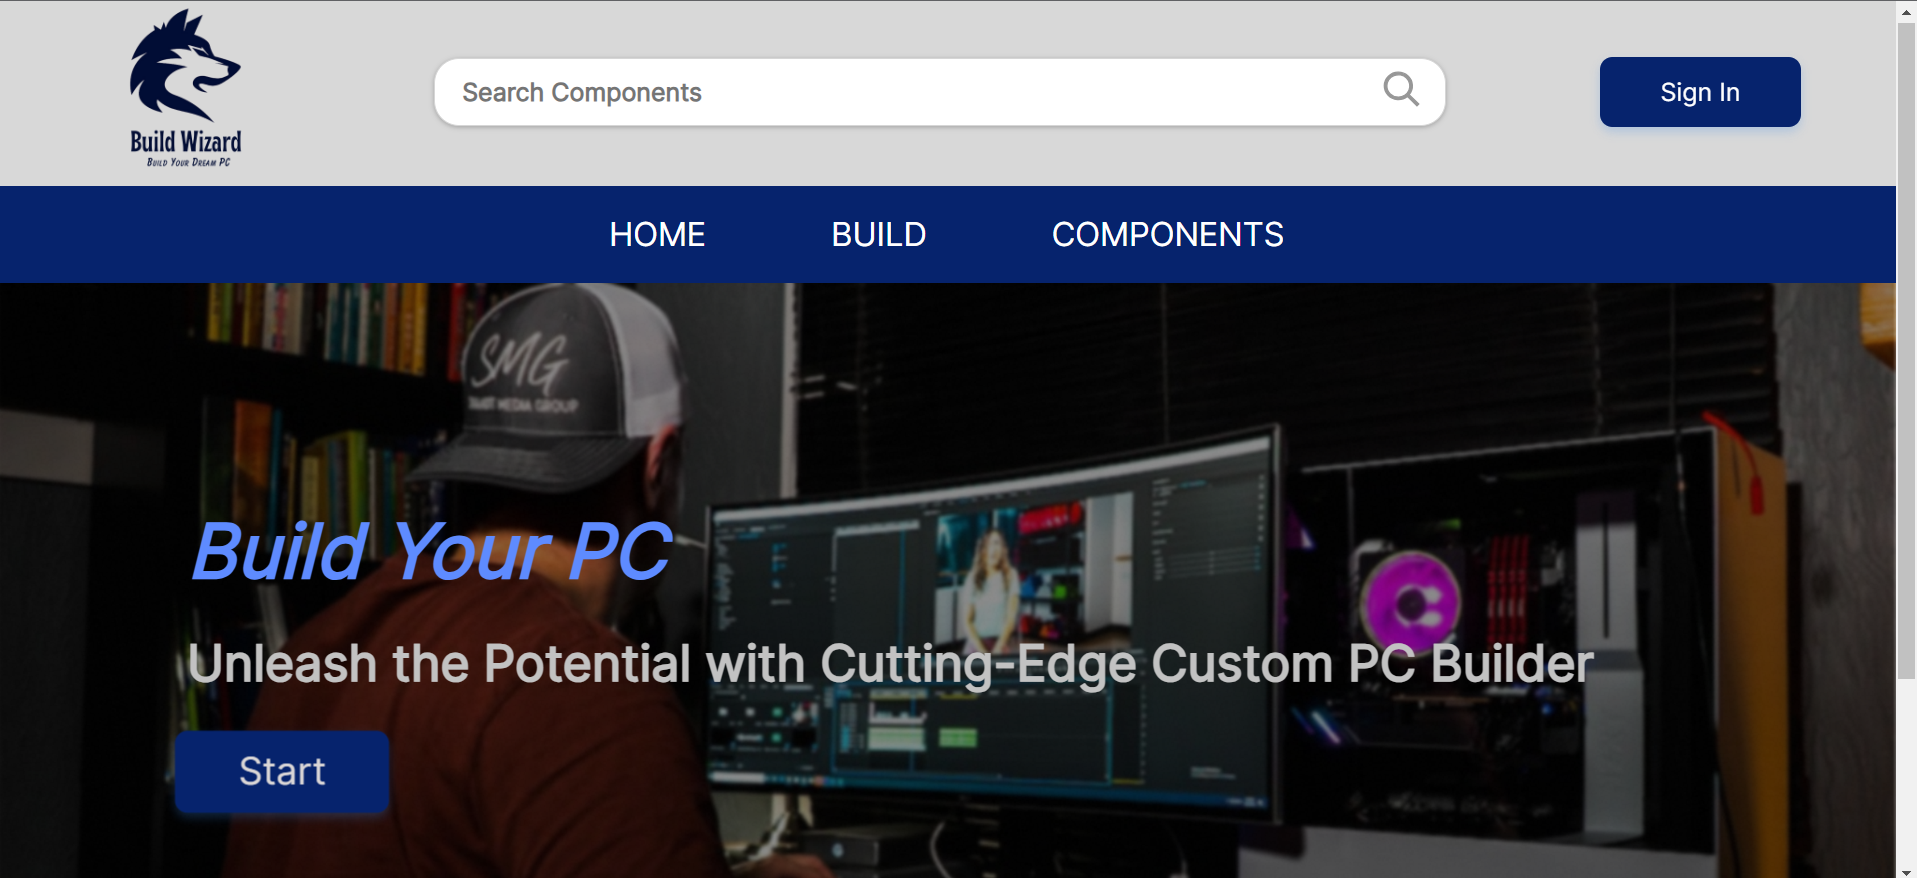
\includegraphics[width=15cm]{Diagrams/UIHOME.png}
      \caption{Interface Design Home page}
      \end{figure}
      
      \newpage
      Below picture shows the UI SignUp page of this website.\\\\
      \begin{figure}[H]
      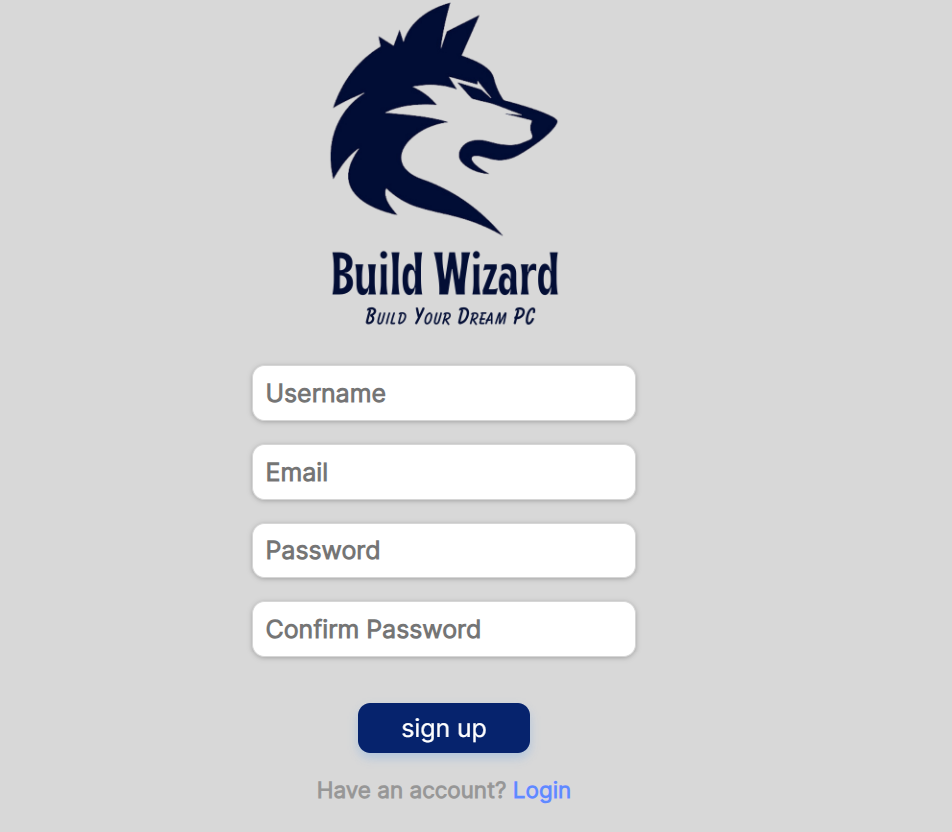
\includegraphics[width=15cm]{Diagrams/UISIGNUP.png}
      \caption{Interface Design SignUp}
      \end{figure}
      \newpage
      Following Picture shows the UI of LogIn on this website.\\\\
      \begin{figure}[H]
      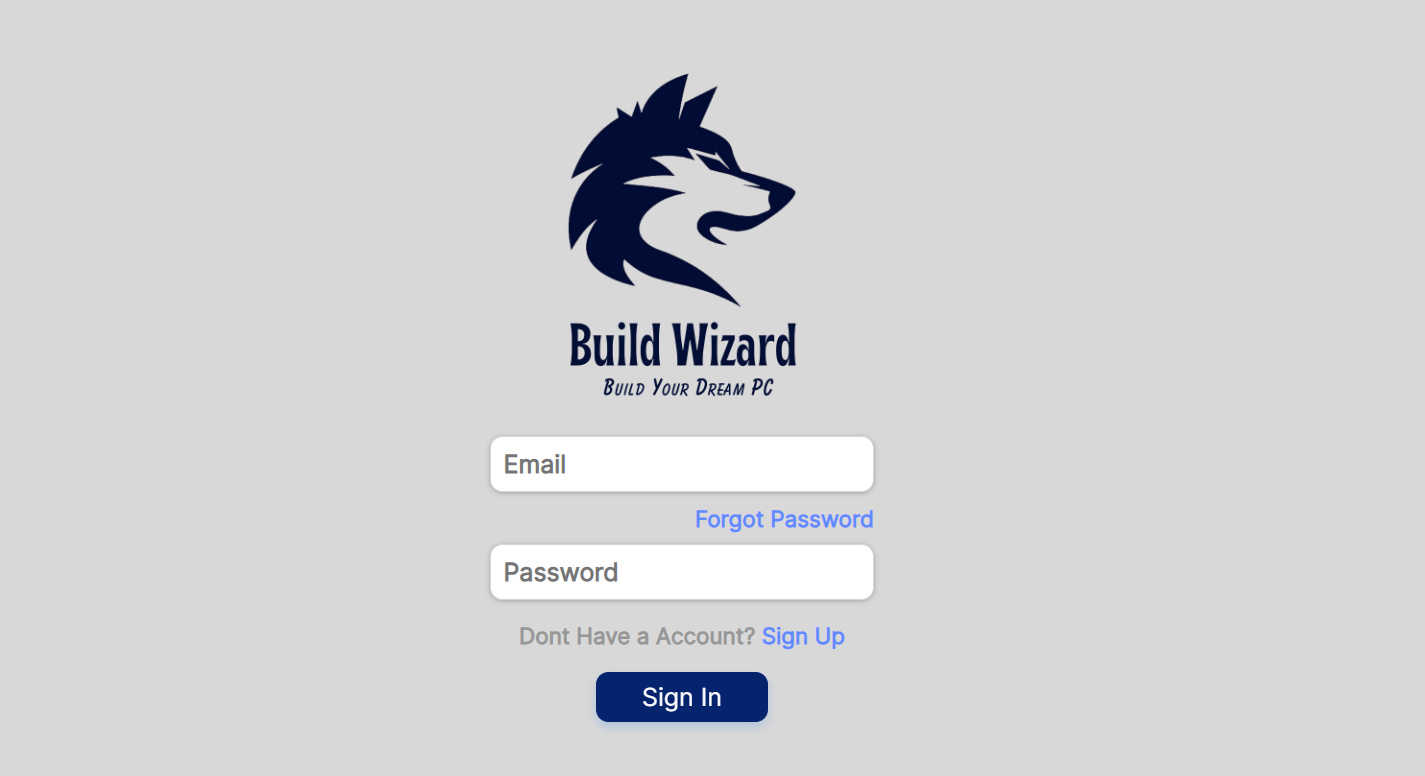
\includegraphics[width=15cm]{Diagrams/UILOGIN.png}
      \caption{Interface Design SignIn}
      \end{figure}
      \subsection{Physical DFD}
      \begin{figure}[H]
         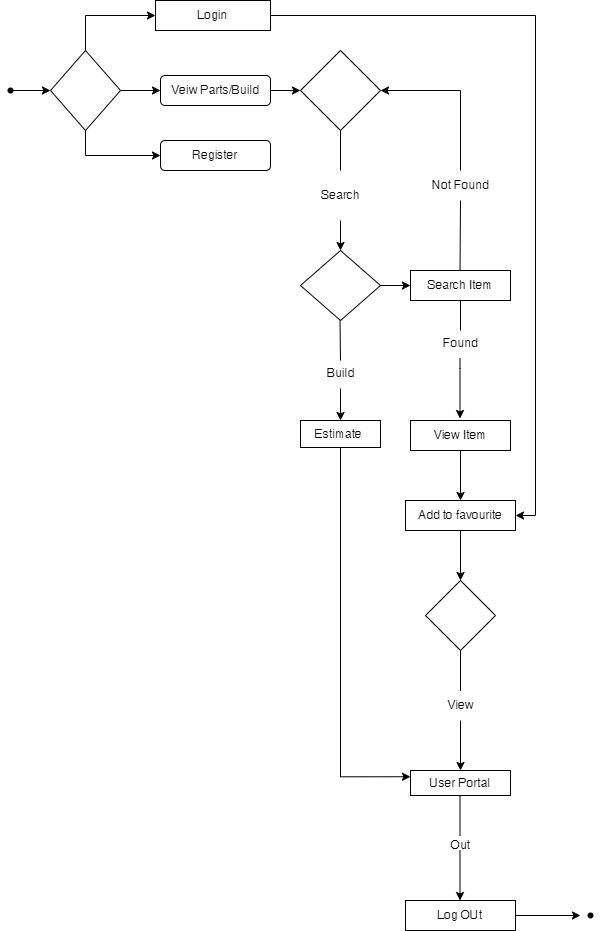
\includegraphics[width=15cm]{Diagrams/physicaldfd.png}
         \caption{Physical DFD diagram}
         \end{figure}
  


      
\chapter{IMPLEMENTATION AND TESTING}


% (20\% of Report Length)

% a. Showcase the output at various intermediate stages of the project pipeline

% b. Use proper data visualizing techniques to present the output

% c. Figures and tables must be accompanied by an explanation
\section{System Development Tools}\textbf{HTML:}\\
HTML, or Hypertext Markup Language, constitutes the backbone of web development by providing the structural foundation for web content. Utilizing a system of tags, HTML defines the arrangement of content elements on a webpage. These tags encapsulate diverse elements, such as headings, paragraphs, images, links, and forms, which compose the web interface. HTML's hierarchical structure reflects the logical flow of information, enhancing accessibility and readability for both users and developers.\\\\
\textbf{PHP:}\\
PHP, or Hypertext Preprocessor, empowers web apps with server-side capabilities for data manipulation, database interaction, and dynamic content generation. It handles form inputs, manages user sessions, and enforces authentication. PHP also performs server-side validation, data processing, and complex backend logic, making it ideal for enhancing platforms like PC part pickers. It seamlessly integrates with JavaScript via AJAX, enabling real-time updates without page reloads, ensuring users receive accurate information and a smooth, interactive experience.\\\\
\textbf{JavaScript:}\\
JavaScript is a versatile scripting language that enables interactivity and dynamic behavior on web pages. It runs directly in the browser, allowing developers to create responsive and engaging user experiences. JavaScript adds a layer of functionality that HTML and CSS alone cannot achieve, making it an essential tool in modern web development.\\\\
\textbf{Figma:}\\
Figma is a cloud-based design tool that plays a vital role in the initial design and prototyping phases of web development. It fosters collaboration among designers and developers, streamlines the design process, and ensures a cohesive and user-centered visual design for the platform.\\\\
\newpage
\textbf{Bootstrap:}\\
Bootstrap is a popular, open-source front-end web framework for designing responsive and mobile-first web pages and applications. It was originally developed by Twitter, and it is now maintained by volunteers through GitHub. Bootstrap provides pre-built design components, CSS (Cascading Style Sheets) frameworks, and JavaScript plugins, making it easier and faster to create consistent, visually appealing, and functional web interfaces.\\\\
\textbf{JQuery:}\\
jQuery is a widely-used JavaScript library that simplifies web development. It provides a collection of pre-built functions and plugins for interacting with HTML documents, handling events, and making asynchronous requests. jQuery streamlines client-side scripting, making it easier to create interactive and dynamic web pages. Its concise syntax and cross-browser compatibility have made it a popular choice for developers seeking to enhance user interfaces and improve the overall user experience on websites and web applications.
% \subsection{Implementation Details of Modules}
\newpage
 \section{Testing}
 \subsection{Test Cases for Unit Testing}
Unit testing is a software testing technique where individual units or components of a software application are tested in isolation to ensure that they function correctly. These units can be functions, methods, classes, or even small modules. Unit testing aims to verify that each unit performs as expected, providing developers with confidence that their code works as intended and catches bugs early in the development process.
\\
\begin{figure}[H]
    \end{figure}
    \begin{table}[H]
        \caption{Unit Test Cases of home/index.php in Build Wizard}
            \label{}
            \begin{tabularx}{\textwidth}{|>{\raggedright\arraybackslash}p{0.3in}|X|>{\raggedright\arraybackslash}p{2in}|X|X|}
                \hline
                Tests & Scenario & Expected Output & Actual Output \\
                \hline
                    1 & GETmethod: favourites =true & User Portal with favourite item & favourite list with description \\
                    \hline
                    2 & GETmethod: search= intel & Shows components of intel & Shows components of intel \\
                    \hline
                    3 & POSTmethod: estimate & Shows estimates of build & shows estimated price\\
                    \hline
    \end{tabularx}
    \end{table}
\newpage
\subsection{Test Cases for System Testing}
Here testing different test cases of authentication system in BuildWizard : Pcpart picker is performed with screenshots as required results:\\
\begin{table}[H]
    \caption{Authentication Test Cases}
        \label{}
        \begin{tabularx}{\textwidth}{|>{\raggedright\arraybackslash}p{0.3in}|X|>{\raggedright\arraybackslash}p{2in}|X|X|}
            \hline
            Tests & Test Cases & Input & Output \\
            \hline
                1 & signup& Email:sirjan2@gmail.com Password:sirjan1234& signup \\
                \hline
                2 & Incorrect  Password in SignIn & Email:sirjan2@gmail.com
                Password:12345679
                Password:12345678 & Password Incorrect \\
                \hline
                3 & Correct Credentials In Login & Email:sirjan2@gmail.com
                Password:sirjan1234 & Redirects to homepage \\
                \hline
\end{tabularx}
\end{table}
 In given below figure we are testing sigin and signup with incorrect and correct authentication.

    \begin{figure}[H]
    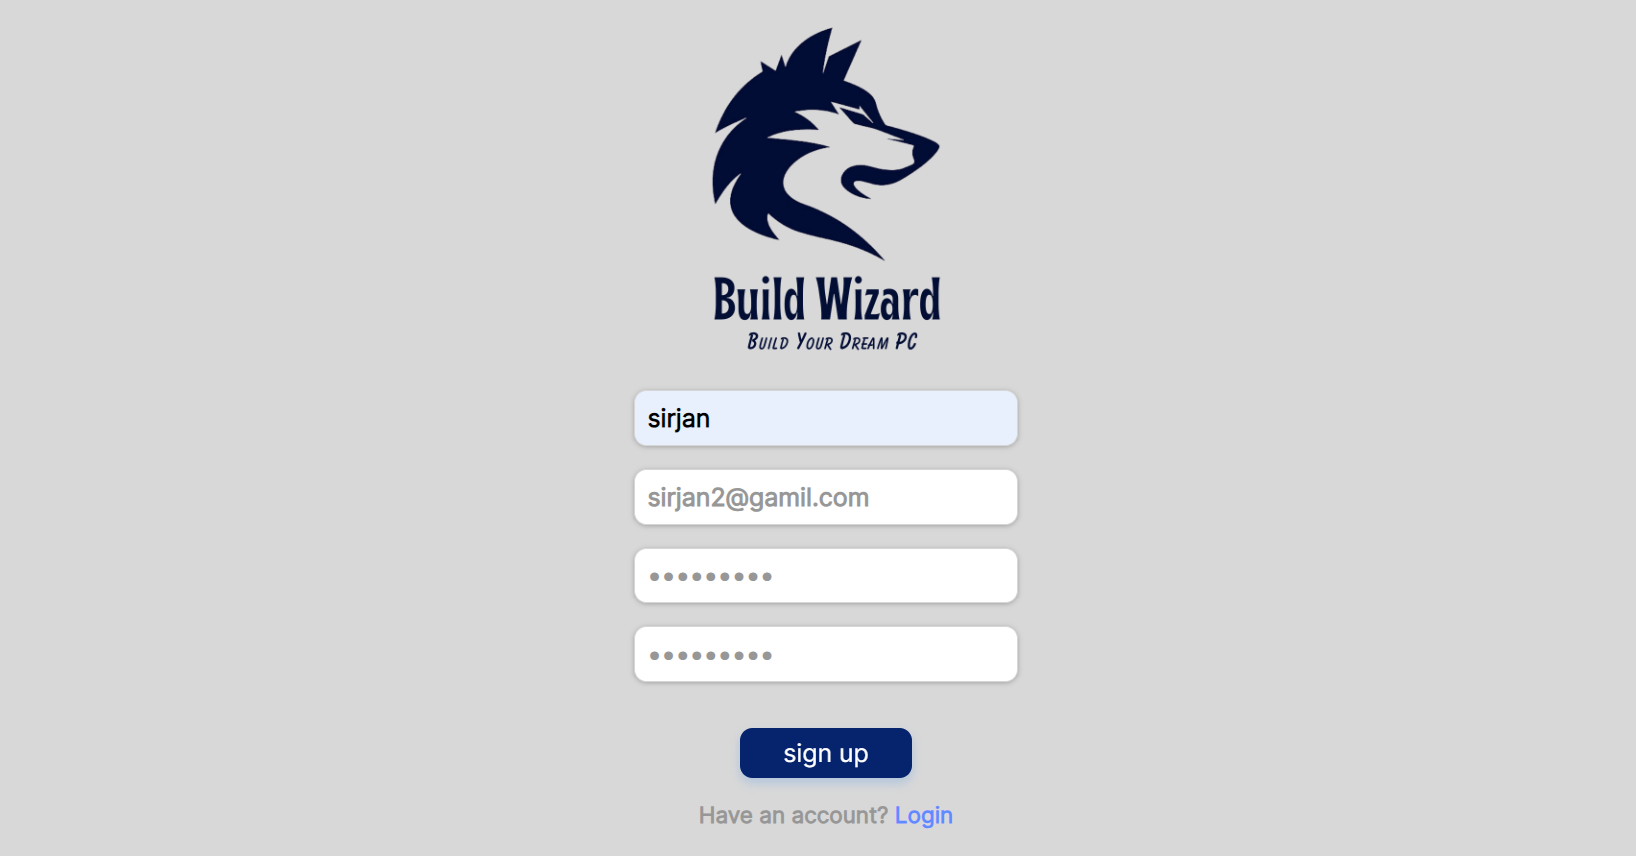
\includegraphics[width=15cm]{Diagrams/sucesssignup.png}
    \caption{Sucessfull SignUp}
    \end{figure}
    \begin{table}[H]
        \caption{Launch Application}
            \label{}
            \begin{tabularx}{\textwidth}{|>{\raggedright\arraybackslash}p{0.3in}|X|>{\raggedright\arraybackslash}p{2in}|X|X|}
                \hline
                Tests & Test Cases & Input & Expected Output & Actual Output \\
                \hline
                    1 & Launch Application & \url{http://localhost/pbw/home/}& Home page & Home page \\
                    \hline
    \end{tabularx}
    \end{table}
    \begin{figure}[H]
    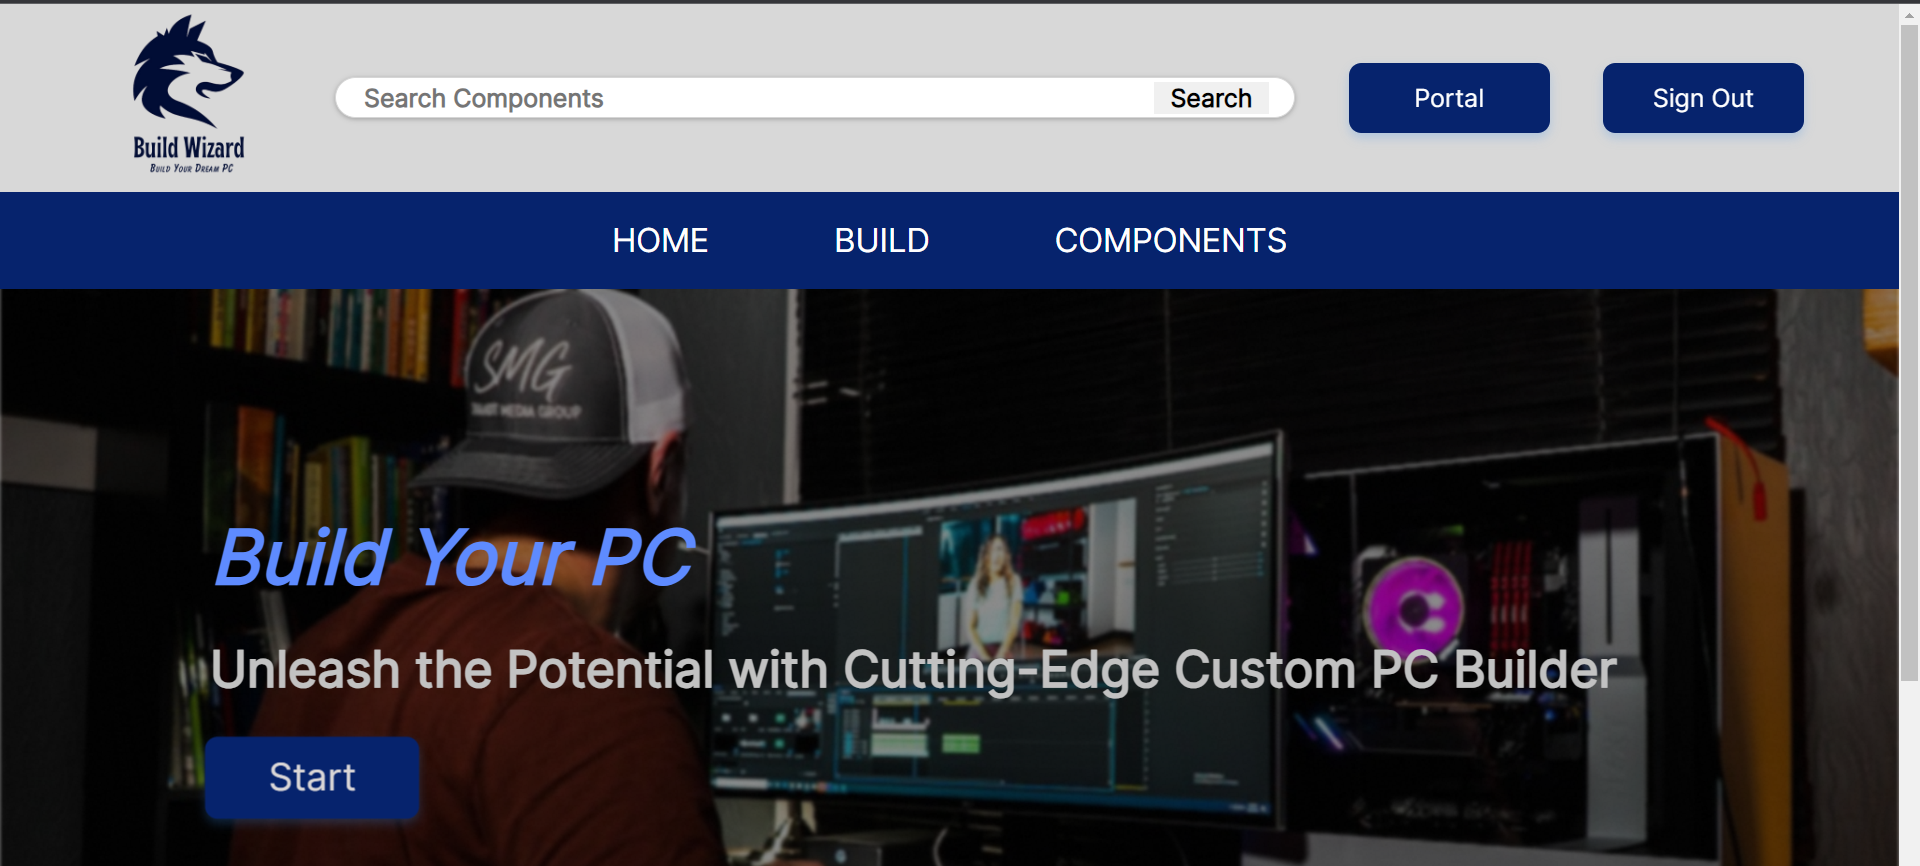
\includegraphics[width=15cm]{Diagrams/sucessloginpage.png}
    \caption{Successful Login}
    \end{figure}
    % admin portal}
    \newpage
        \begin{table}[H]
            \caption{Add component by Admin}
                \label{}
                \begin{tabularx}{\textwidth}{|>{\raggedright\arraybackslash}p{0.3in}|X|>{\raggedright\arraybackslash}p{2in}|X|X|}
                    \hline
                    Tests & Test Cases & Input & Expected Output & Actual Output \\
                    \hline
                        1 & Add components/Manage CPU  & \url{http://localhost/pbw/adminportal/?manage=cpu} & Add product details in form  & opens cpu form  \\
                        \hline
                        2 & Delete components/Manage CPU & \url{http://localhost/pbw/adminportal/?manage=cpu}
                        & Manage Product list & Remove unwanted components\\
                        \hline
        \end{tabularx}
        \end{table}
        \begin{figure}[H]
            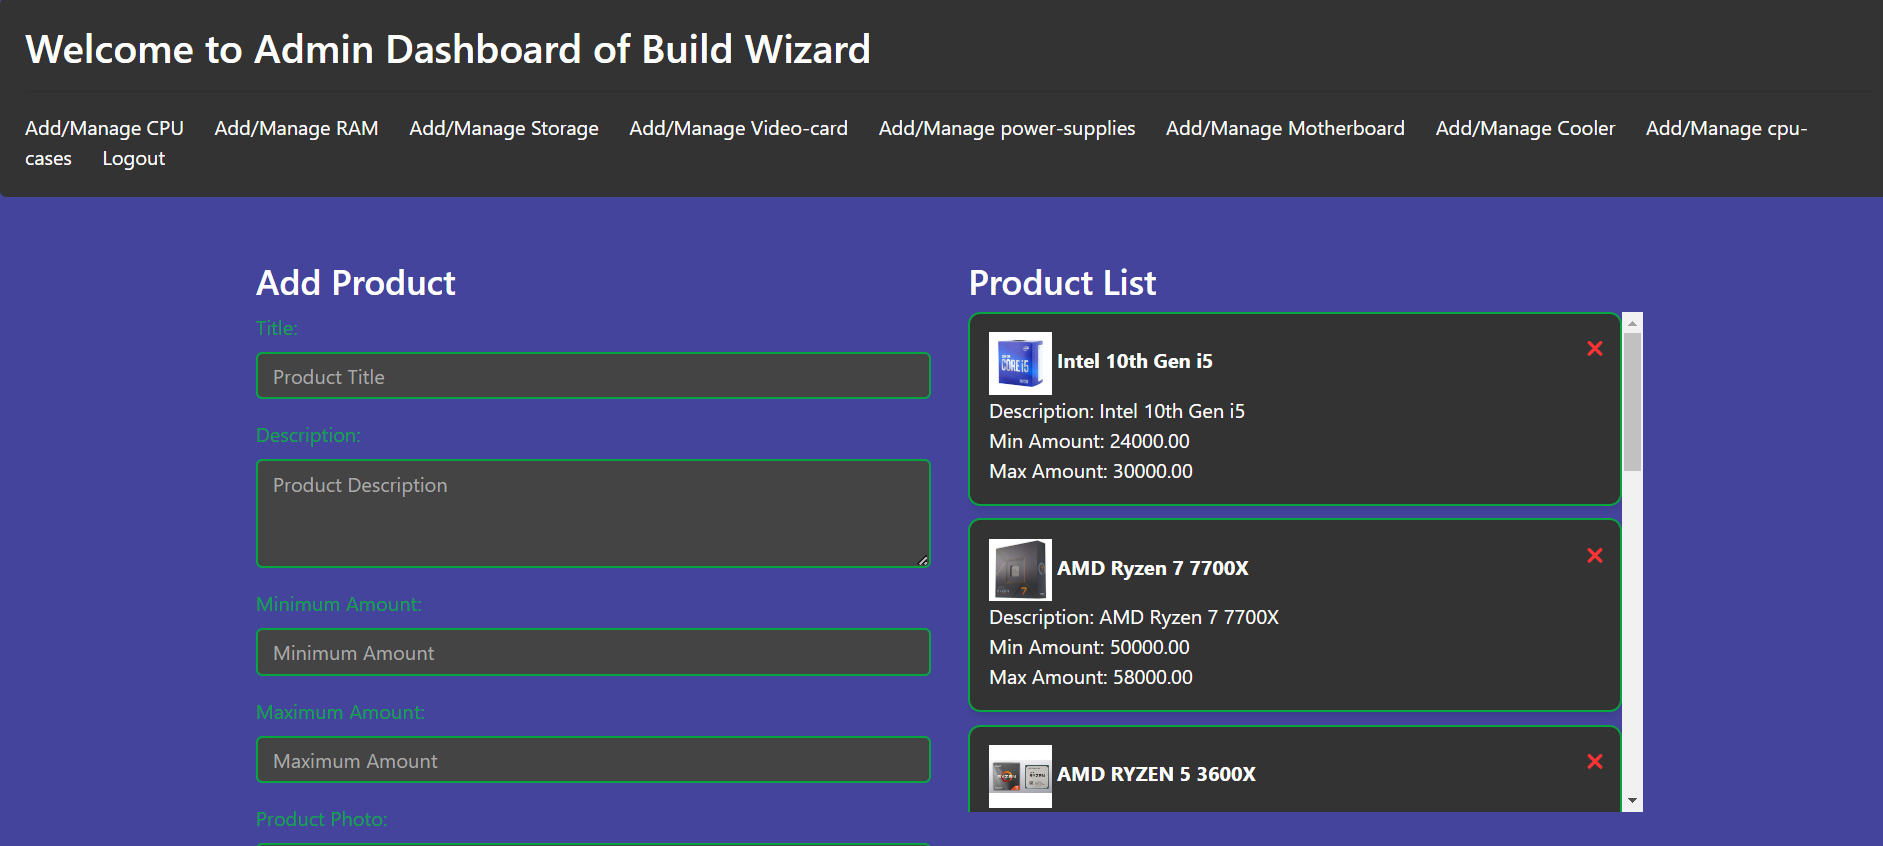
\includegraphics[width=15cm]{Diagrams/admin_portal.png}
            \caption{Add component by Admin}
            \end{figure}
        % components
        \newpage
            \begin{table}[H]
                \caption{Component page}
                    \label{}
                    \begin{tabularx}{\textwidth}{|>{\raggedright\arraybackslash}p{0.3in}|X|>{\raggedright\arraybackslash}p{2in}|X|X|}
                        \hline
                        Tests & Test Cases & Input & Expected Output & Actual Output \\
                        \hline
                            1 & Show components & \url{http://localhost/pbw/components/} & Components & Shows components  \\
                            \hline
                           2 & Component: RAM  &\url{http://localhost/pbw/products/?component=ram}& shows list of ram& ram details \\
                           \hline
            \end{tabularx}
            \end{table}
            \begin{figure}[H]
                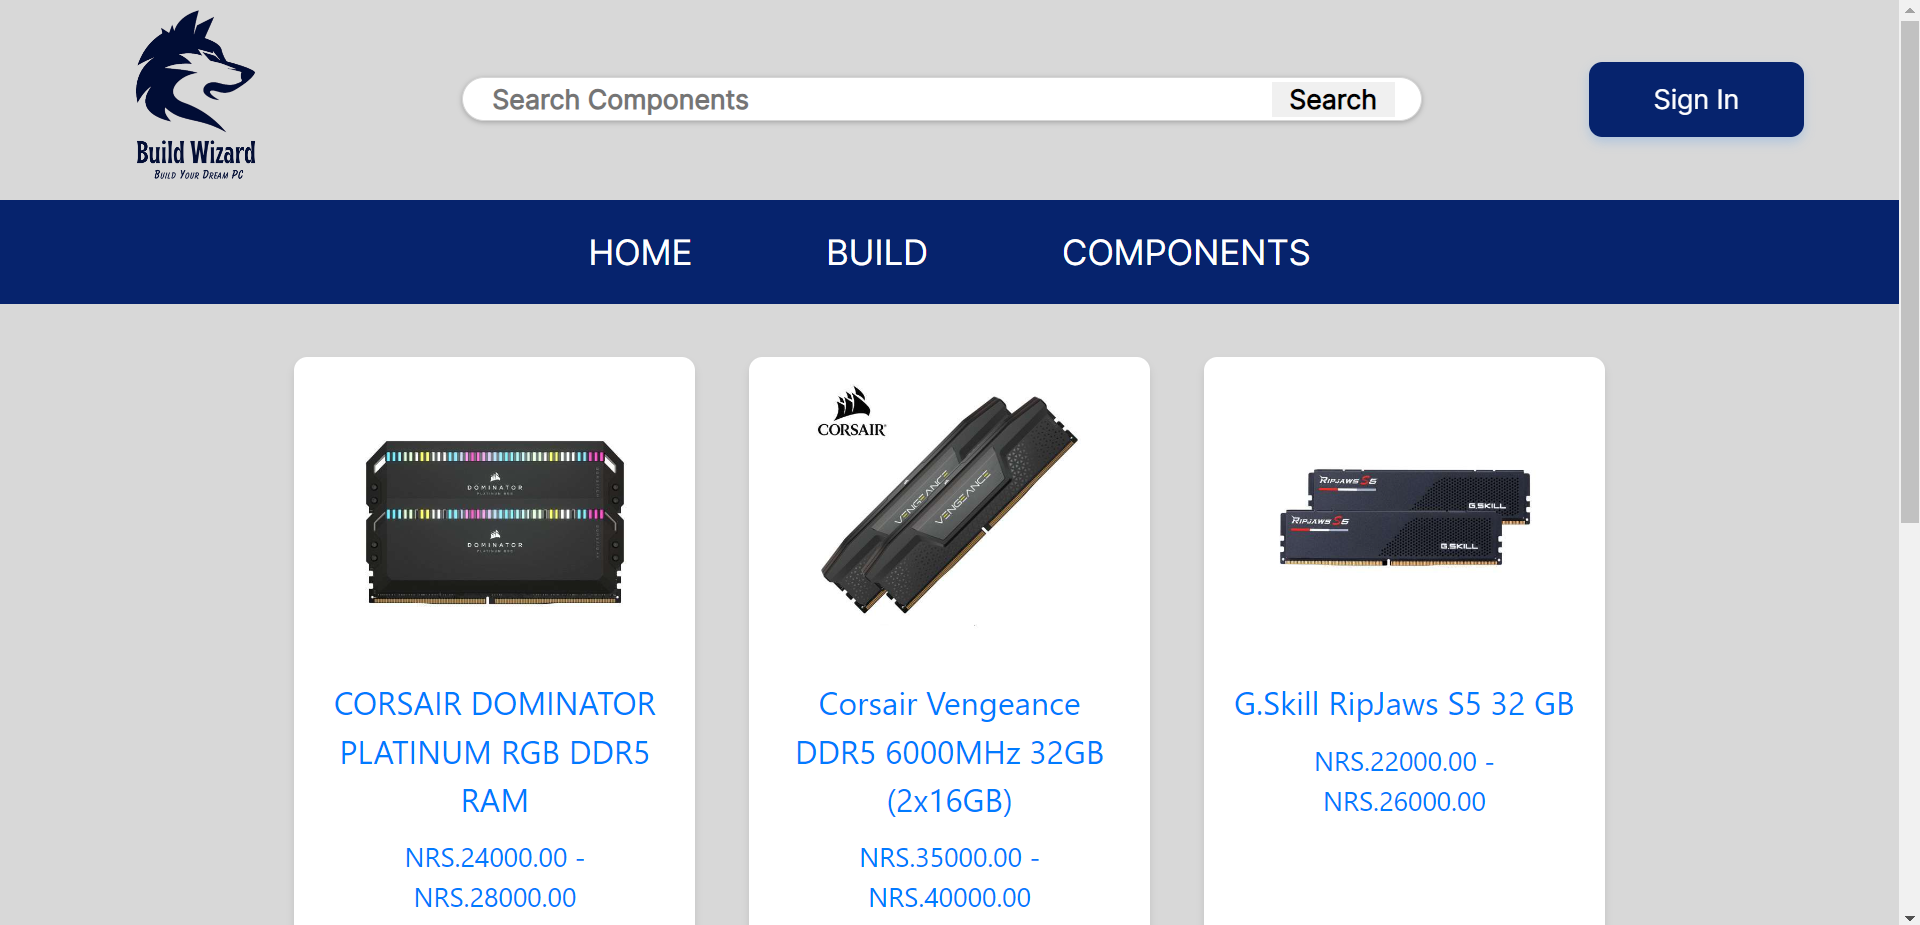
\includegraphics[width=15cm]{Diagrams/rams.png}
                \caption{Components}
                \end{figure}
        

% \subsection{Test Cases for Unit Testing}
% \subsection{Test Cases for System Testing}
\chapter{CONCLUSION AND FUTURE RECOMMENDATION}
\section{Lesson Learnt/Outcome}
\subsection{Home Page}
At the top of the home page, there's a header section that includes the project logo, navigation menu, and user login/signup options. This section provides easy access to different parts of the platform and allows users to log in or create an account.
\begin{figure}[H]
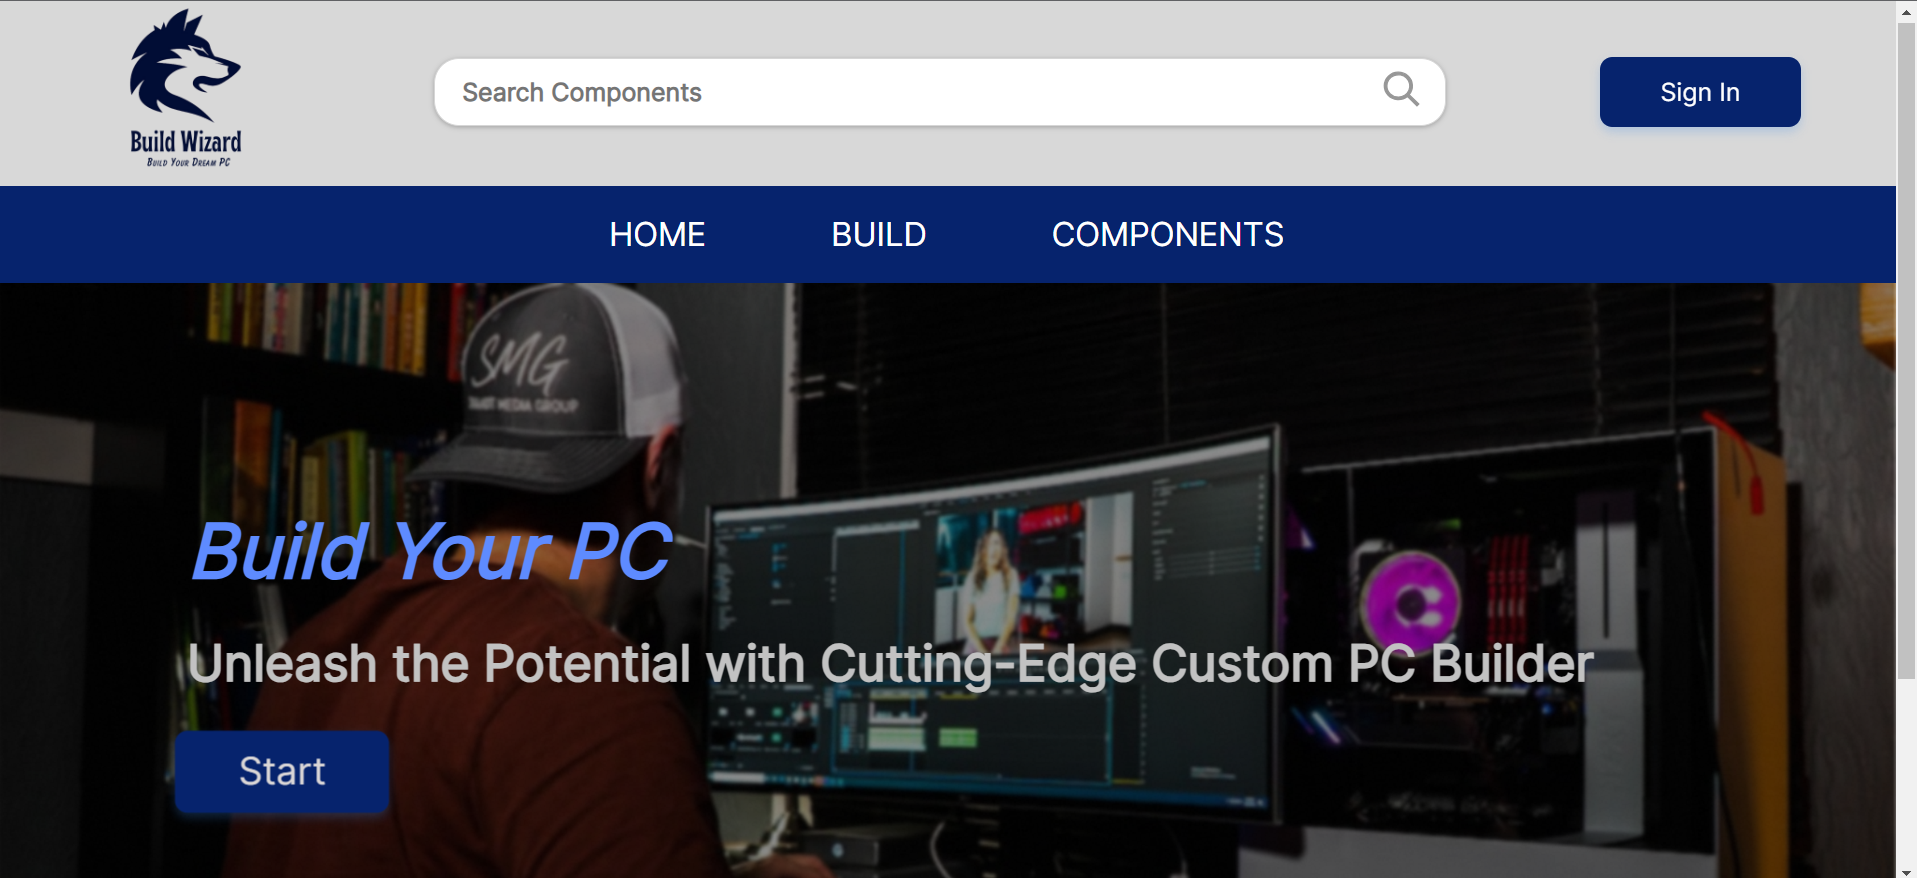
\includegraphics[width=15cm]{Diagrams/UIHOME.png}
\caption{Home Page}
\end{figure}
\newpage
\subsection{Build Page}
A Build Page within the context of the Build Wizard :PC part picker project refers to a dedicated section of the platform where users can create and customize their own PC configurations. This page allows users to select various computer components, such as processors, graphics cards, memory modules, storage devices, and more, to assemble a complete and functional computer system tailored to their specific needs and preferences.
\begin{figure}[H]
\centering
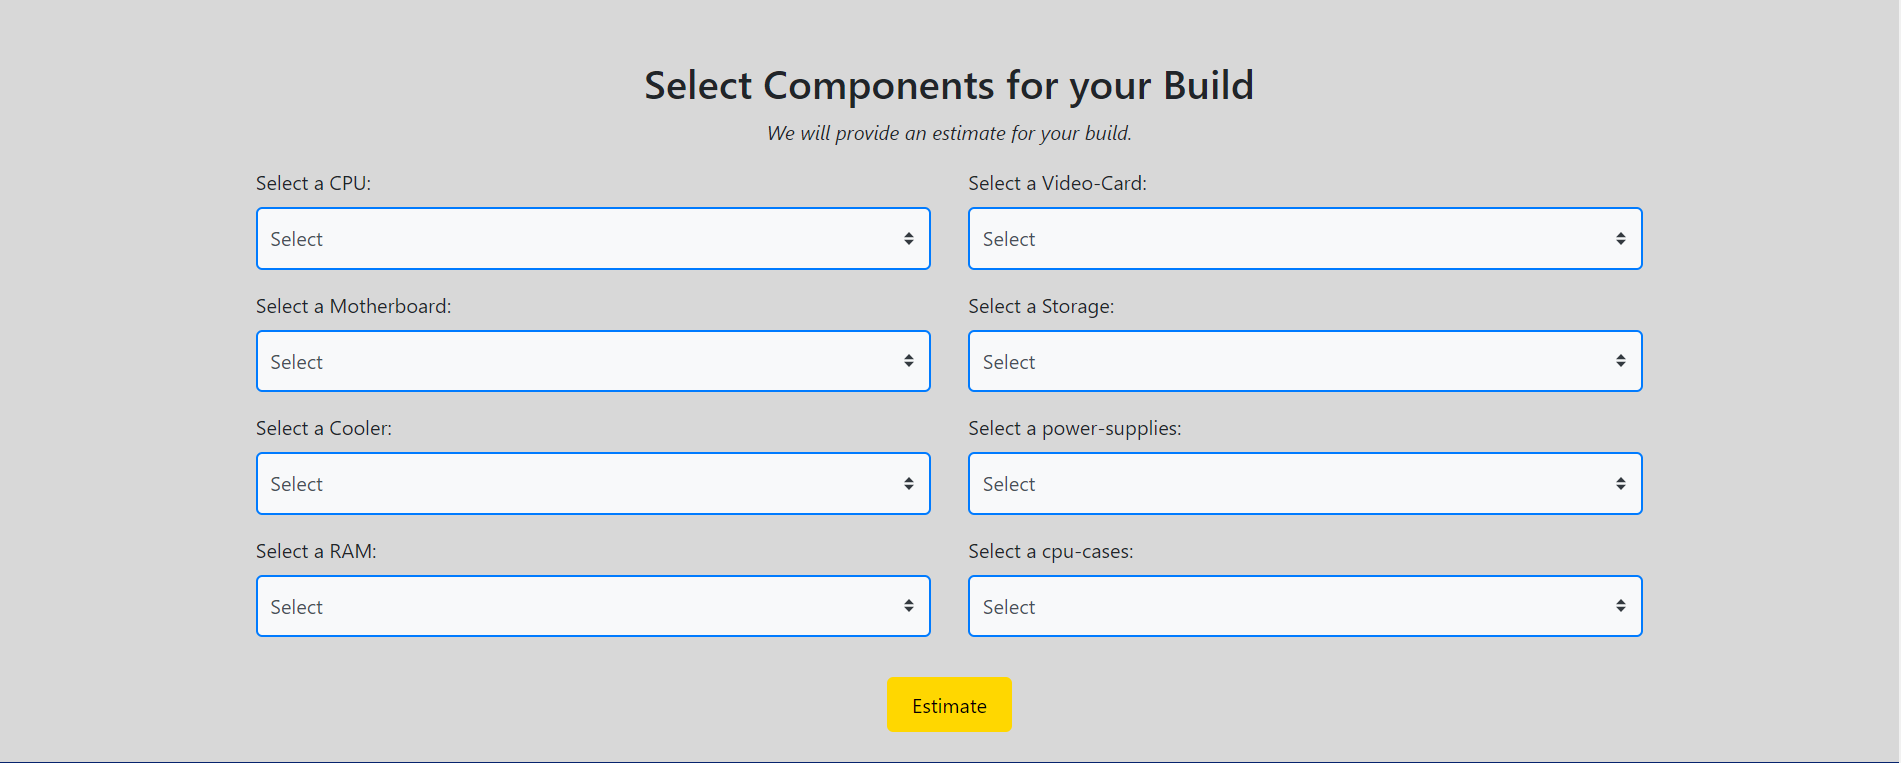
\includegraphics[width=16cm]{Diagrams/newbuildpage.png}
\caption{Build Page}
\end{figure}
\subsection{Components Page}
The "Components" page for this project, focusing on building a user-friendly platform for veiwing pc components and their information. It's crucial to design this page to be intuitive, informative, and visually appealing to provide a better experience.
\begin{figure}[H]
    \centering
    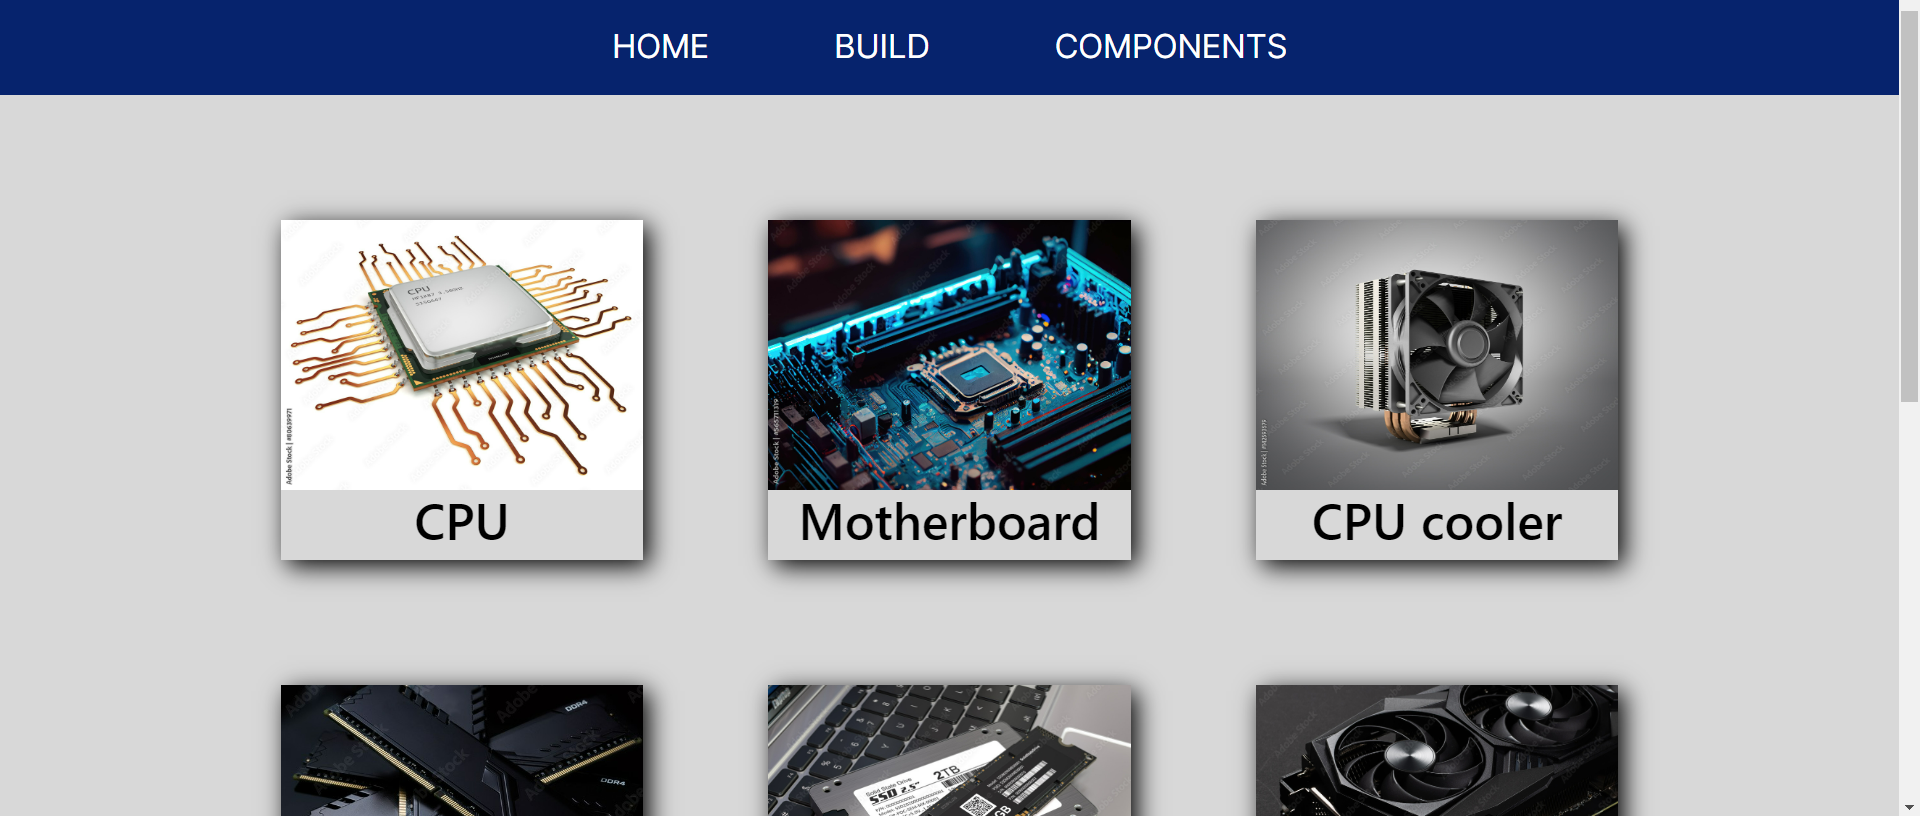
\includegraphics[width=16cm]{Diagrams/components.png}
    \caption{component Page}
    \end{figure}
\subsection{Admin Portal}
The admin portal for this project serves as a centralized interface accessible to authorized administrators, allowing them to manage componets for the webpage.
\begin{figure}[H]
    \centering
    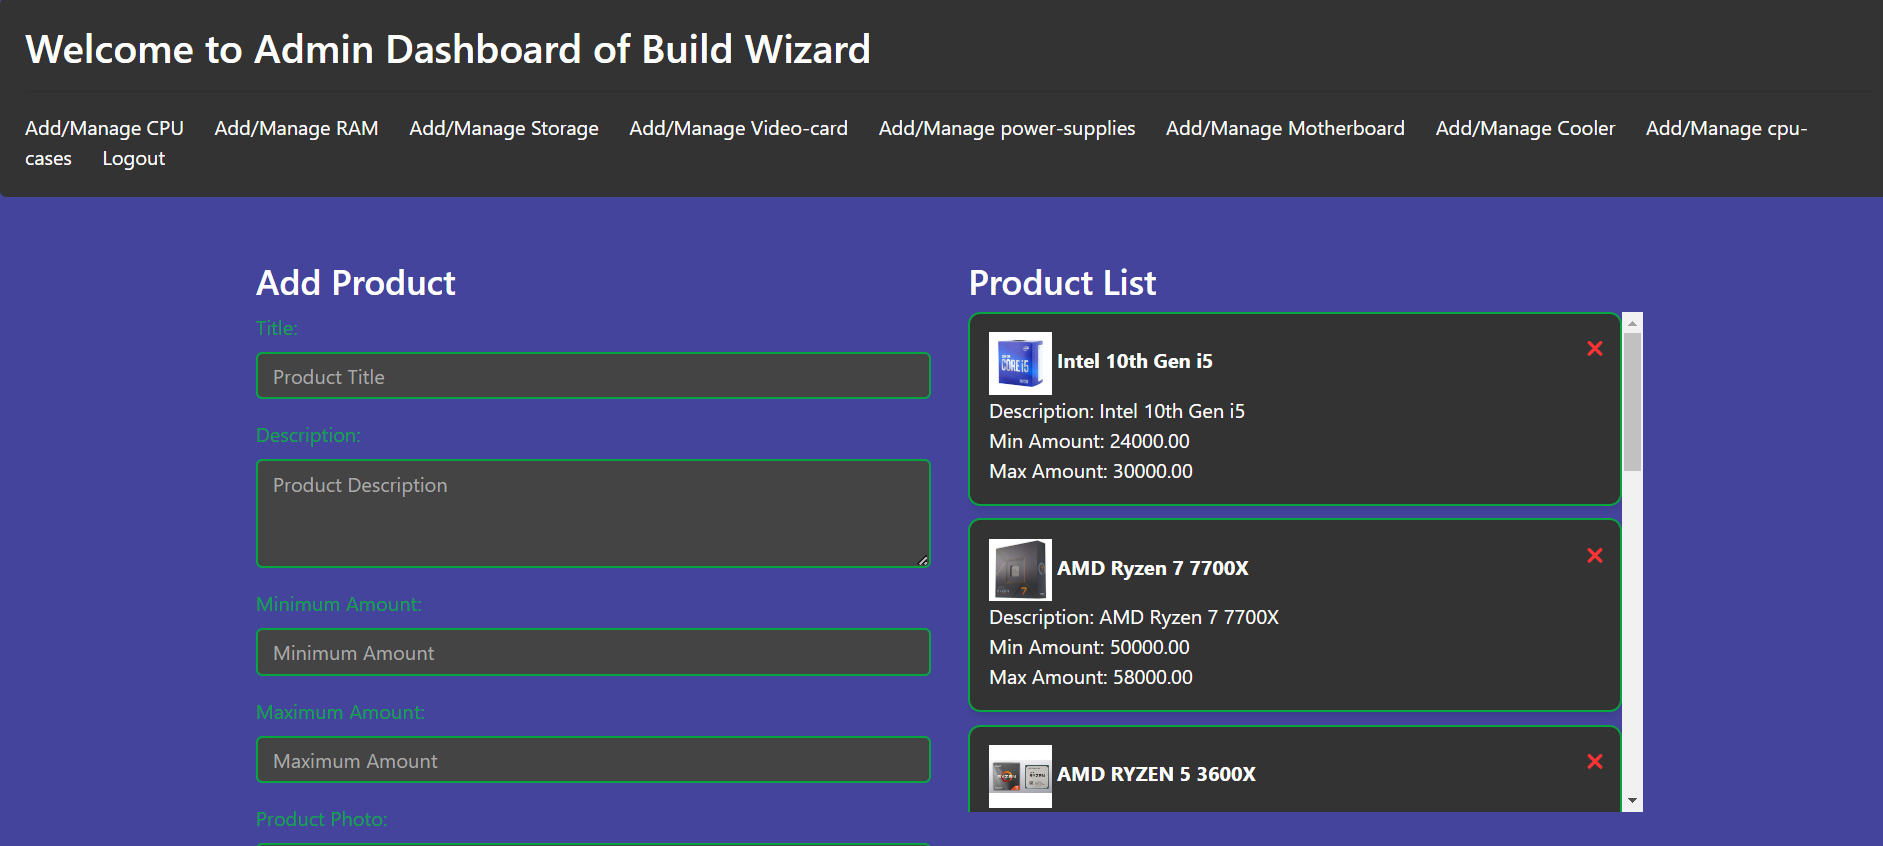
\includegraphics[width=16cm]{Diagrams/admin_portal.png}
    \caption{Admin Page}
    \end{figure}
\subsection{Sign-in Page}
\begin{figure}[H]
    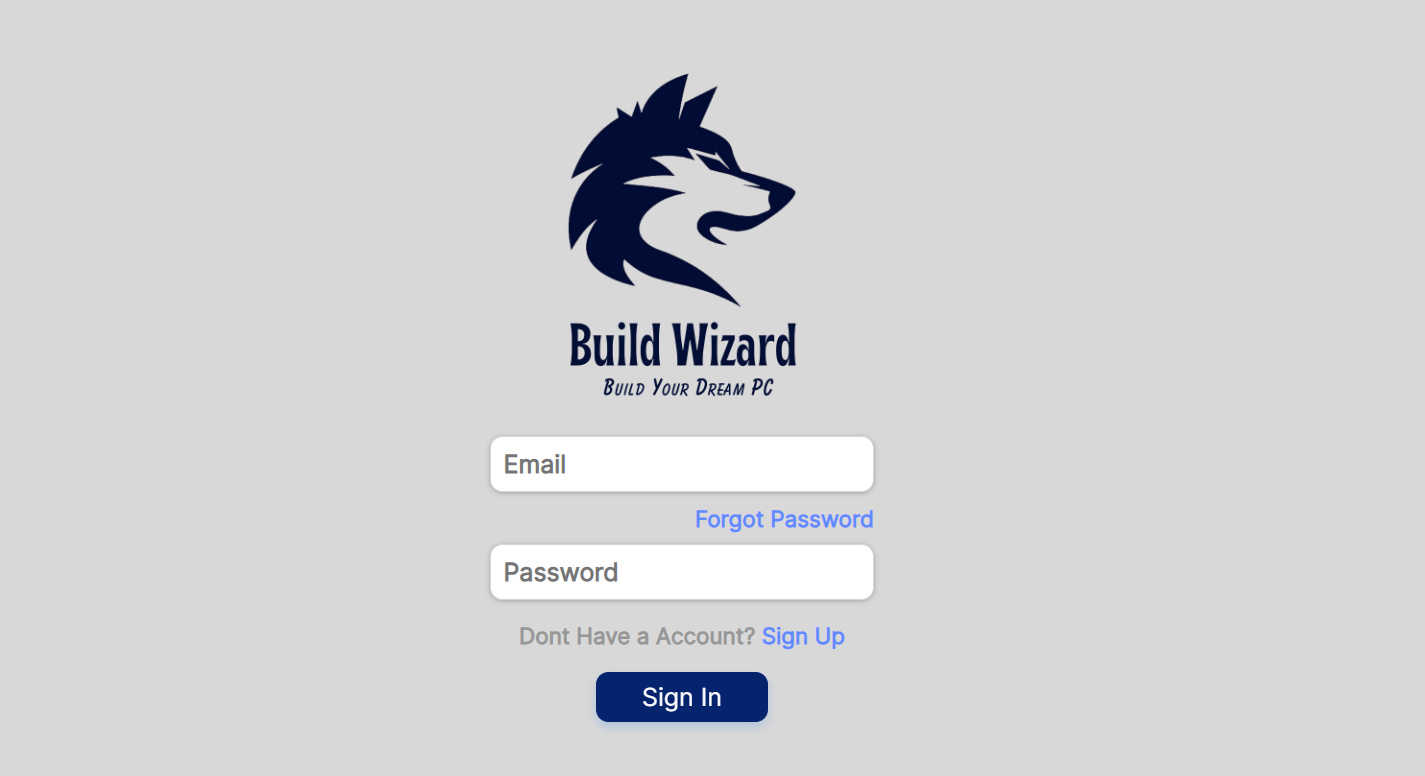
\includegraphics[width=16cm]{Diagrams/UILOGIN.png}
    \caption{SignIn Page}
    \end{figure}
    \subsection{Incorrect Password}
    \begin{figure}[H]
        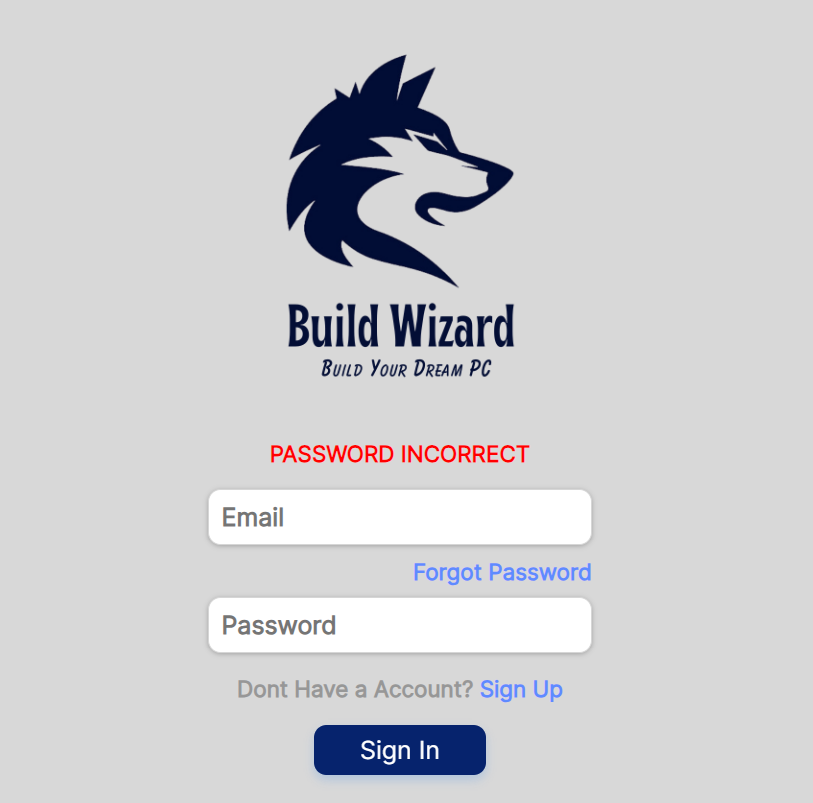
\includegraphics[width=15cm]{Diagrams/incorrect password.png}
        \caption{Incorrect Password}
        \end{figure}
\subsection{Sign-up Page}
\begin{figure}[H]
    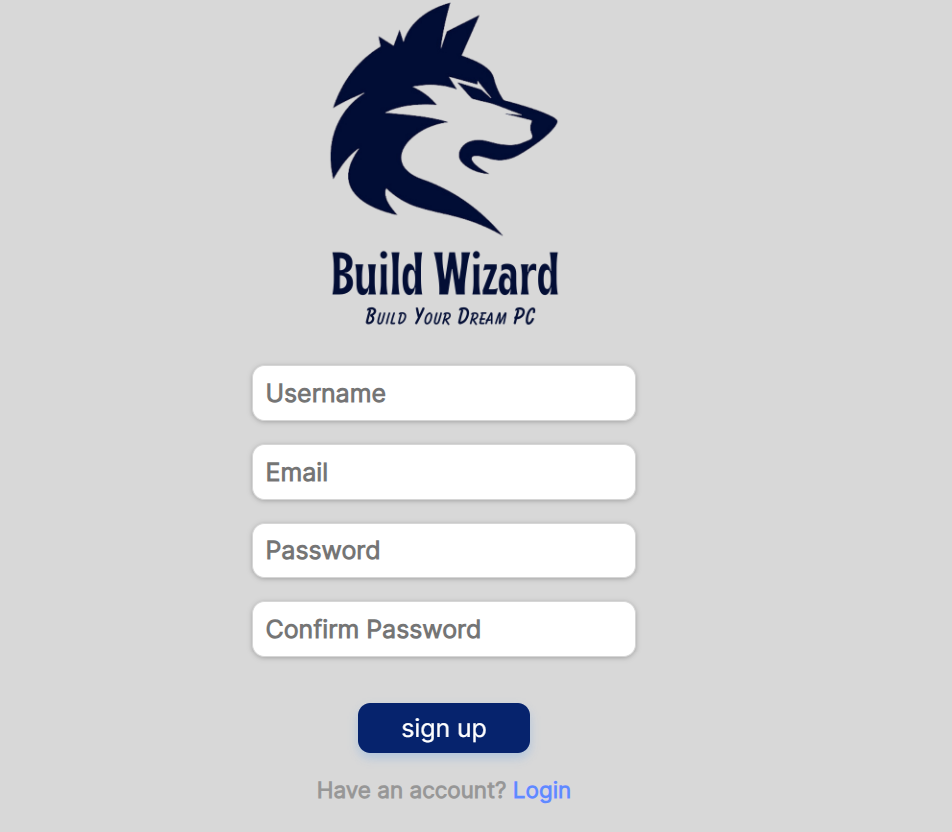
\includegraphics[width=16cm]{Diagrams/UISIGNUP.png}
    \caption{SignUp Page}
    \end{figure}
    \subsection{Searching Page}
\begin{figure}[H]
    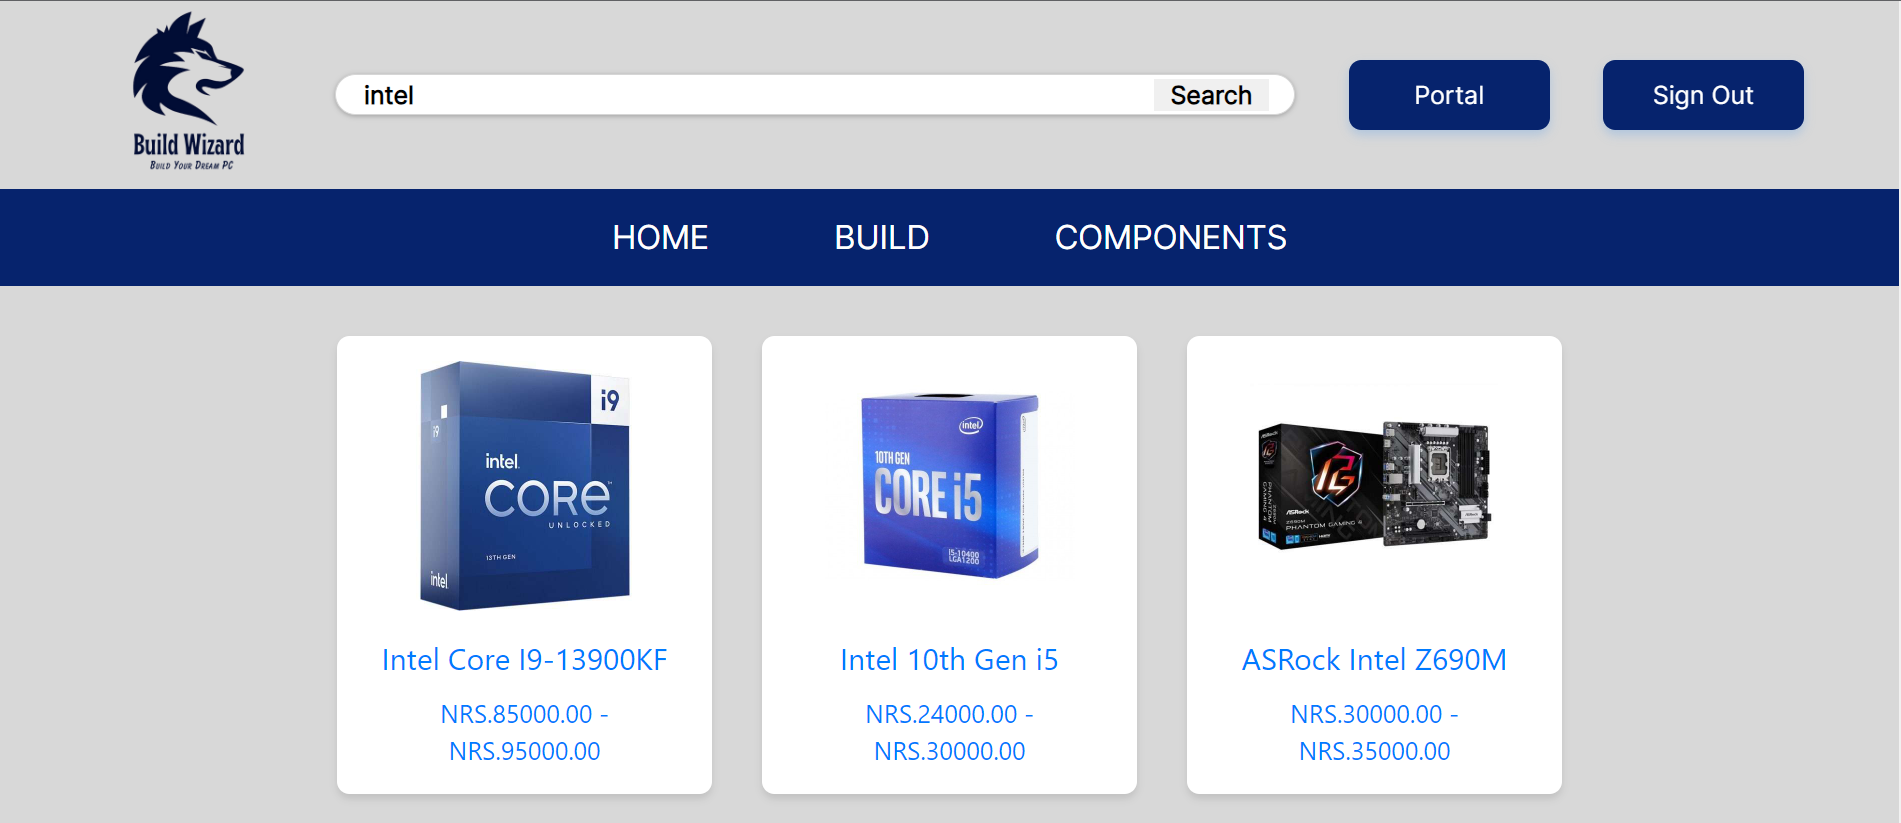
\includegraphics[width=16cm]{Diagrams/searching.png}
    \caption{Searching Page}
    \end{figure}
\section{Conclusion}
In conclusion, the Build Wizard project is an innovative online platform tailored for the Nepalese PC building community. It addresses compatibility challenges and facilitates price comparisons. This localized solution simplifies the PC building process, promoting informed decisions and enhancing the overall PC building experience in Nepal.
\section{Future Recommendations}
\begin{itemize}
    \item \textbf{Vendors:} In future ,Local vendors can feature products.
    \item \textbf{Ordering System:} Odering and delivary system can be integrated.
    \item \textbf{Mobile Accessibility:} System will accessible and user-friendly on mobile devices, as many users may prefer to use it on smartphones or tablets.
    \item \textbf{Offline Customization:} This would allow users to customize the system and use it even when they don't have an internet connection. This can be particularly useful in situations where a stable internet connection is not guaranteed.
\end{itemize}
% \chapter{Discussion and Analysis}
% The PC part picker project is an endeavor aimed at simplifying the intricate process of selecting and configuring PC components. This project's significance lies in the growing complexity of PC components and the need for a user-friendly platform to guide users through the selection process.

% In terms of technology, the project integrates HTML, CSS, JavaScript, PHP, MySQL, and Figma. These tools collectively enable the creation of a dynamic and responsive user interface. However, a significant technical challenge involves developing compatibility algorithms that accurately assess the viability of component combinations. Real-time data synchronization with external sources for current component information also poses a technical hurdle.

% The platform's functionality encompasses various aspects, from component search and filtering to compatibility analysis and configuration creation. Notably, user engagement is fostered through interactive features driven by JavaScript and the provision of user reviews and feedback sections.

% User experience is central to the project's success. A user-friendly interface that facilitates easy navigation is vital. Real-time updates ensure users access the latest information. Addressing data privacy concerns is crucial to maintain user trust.

% Looking forward, the project's adaptability is key. As the PC component market evolves, the platform should seamlessly integrate new components and technologies. User feedback should guide iterative development, ensuring continuous enhancement of functionalities.

% In conclusion, the PC part picker project amalgamates technology, user experience, and iterative development. Through the collaboration of HTML, CSS, JavaScript, PHP, MySQL, and Figma, the platform aims to guide users through the complexity of PC component selection, thereby simplifying the process and empowering users to build their ideal PC configurations.



% ================================Appendices Setup================================================


\begin{appendices}
\renewcommand\thechapter{A}
\renewcommand\thefigure{\thechapter.\arabic{figure}}
\chapter*{APPENDIX A}
\addtocontents{toc}{\textbf{APPENDIX A}}
\section{Project Schedule}
Below is the Gantt chart of our project Schedule. We have planned to perfrom these specific tasks between these time frames.
\begin{figure}[H]
    \centering
        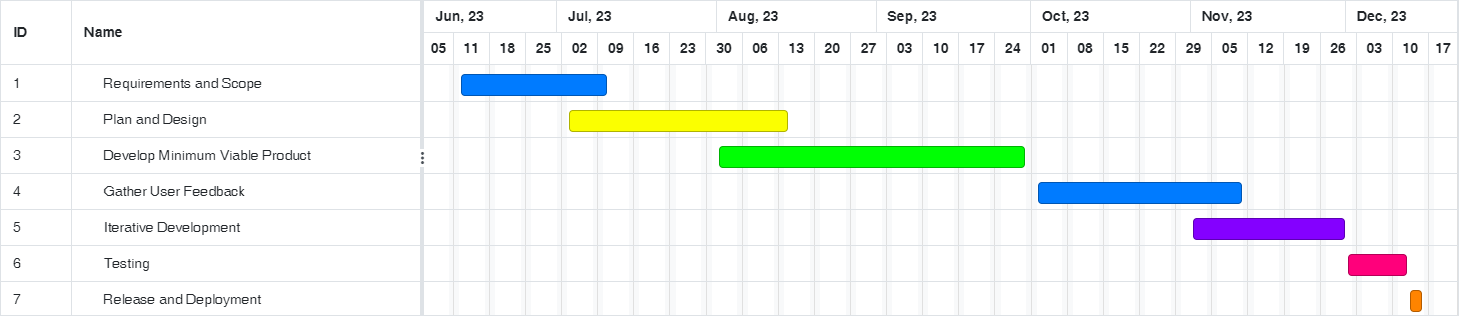
\includegraphics[width=400px]{Diagrams/Gantt_Chart.png}
    \caption{Gantt Chart of Schedule}
\end{figure}

\newpage
\section{Setup Guide to run BuildWizard Locally}
\begin{enumerate}
    \item \textbf{Prerequisite:}
    \begin{enumerate}
        \item XAMPP
        \item Operating System that support XAMPP.
        \item Internet Connection for CDN libraries.
        \item Project Files Cloned from Git Hub.
    \end{enumerate}
    \item Clone Repo in htdocs/\
    \begin{verbatim}
     git clone https://github.com/sujalmhrzn/BuildWizard
    \end{verbatim}
    \item Open PhpMyAdmin by going into \url{http://localhost/phpmyadmin}
    \item Create Database BuildWizard
    \item Import Database sql file from folder cloned using Import button located in navbar.
    \item Open XAMPP Control Panel.
    \item Start Apache and MySQL Servers.
    \item Run it on http://localhost/ Build Wizard directory.
\end{enumerate}
\section{Running Hosted Build Wizard}
\begin{enumerate}
    \item Open Mobile/Desktop Browser .
    \item Go to \url{https://github.com/sujalmhrzn/BuildWizard}
\end{enumerate}
\newpage
\section{MySQL Connection in our Build Wizard PHP}
\vspace{1cm}
\begin{lstlisting}
    <?php
    $servername = "localhost";
    $username = "root";
    $password = "";
    $dbname = "BuildWizard";

    $conn = new mysqli($servername, $username, $password, $dbname);

    if ($conn->connect_error) {
        die("Connection failed: " . $conn->connect_error);
    }
    ?>
    \end{lstlisting}
    \newpage
    \section{Database}
    In the context of the PC part picker project, a database is a structured and organized collection of digital information. It stores essential data such as user profiles and component details.\\
Following figures shows database of users.
\begin{figure}[H]
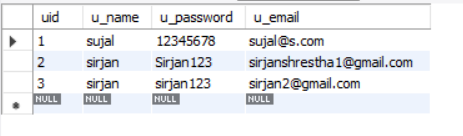
\includegraphics[width=15cm]{Diagrams/Users Database.png}
\caption{User Database}
\end{figure}
Following figures shows components database
\begin{figure}[H]
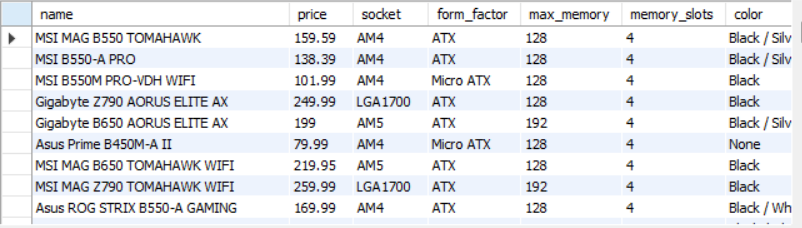
\includegraphics[width=16cm]{Diagrams/motherboard.png}
\caption{Motherboard Database}
\end{figure}
\begin{figure}[H]
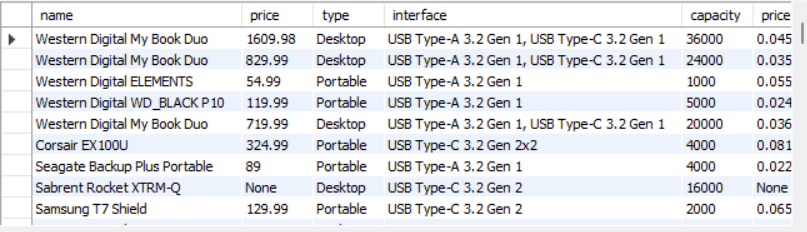
\includegraphics[width=16cm]{Diagrams/External HDD.png}
\caption{External HDD}
\end{figure}

\newpage
\section{Supervisor Consultation Form}
\begin{figure}[H]
    \centering
    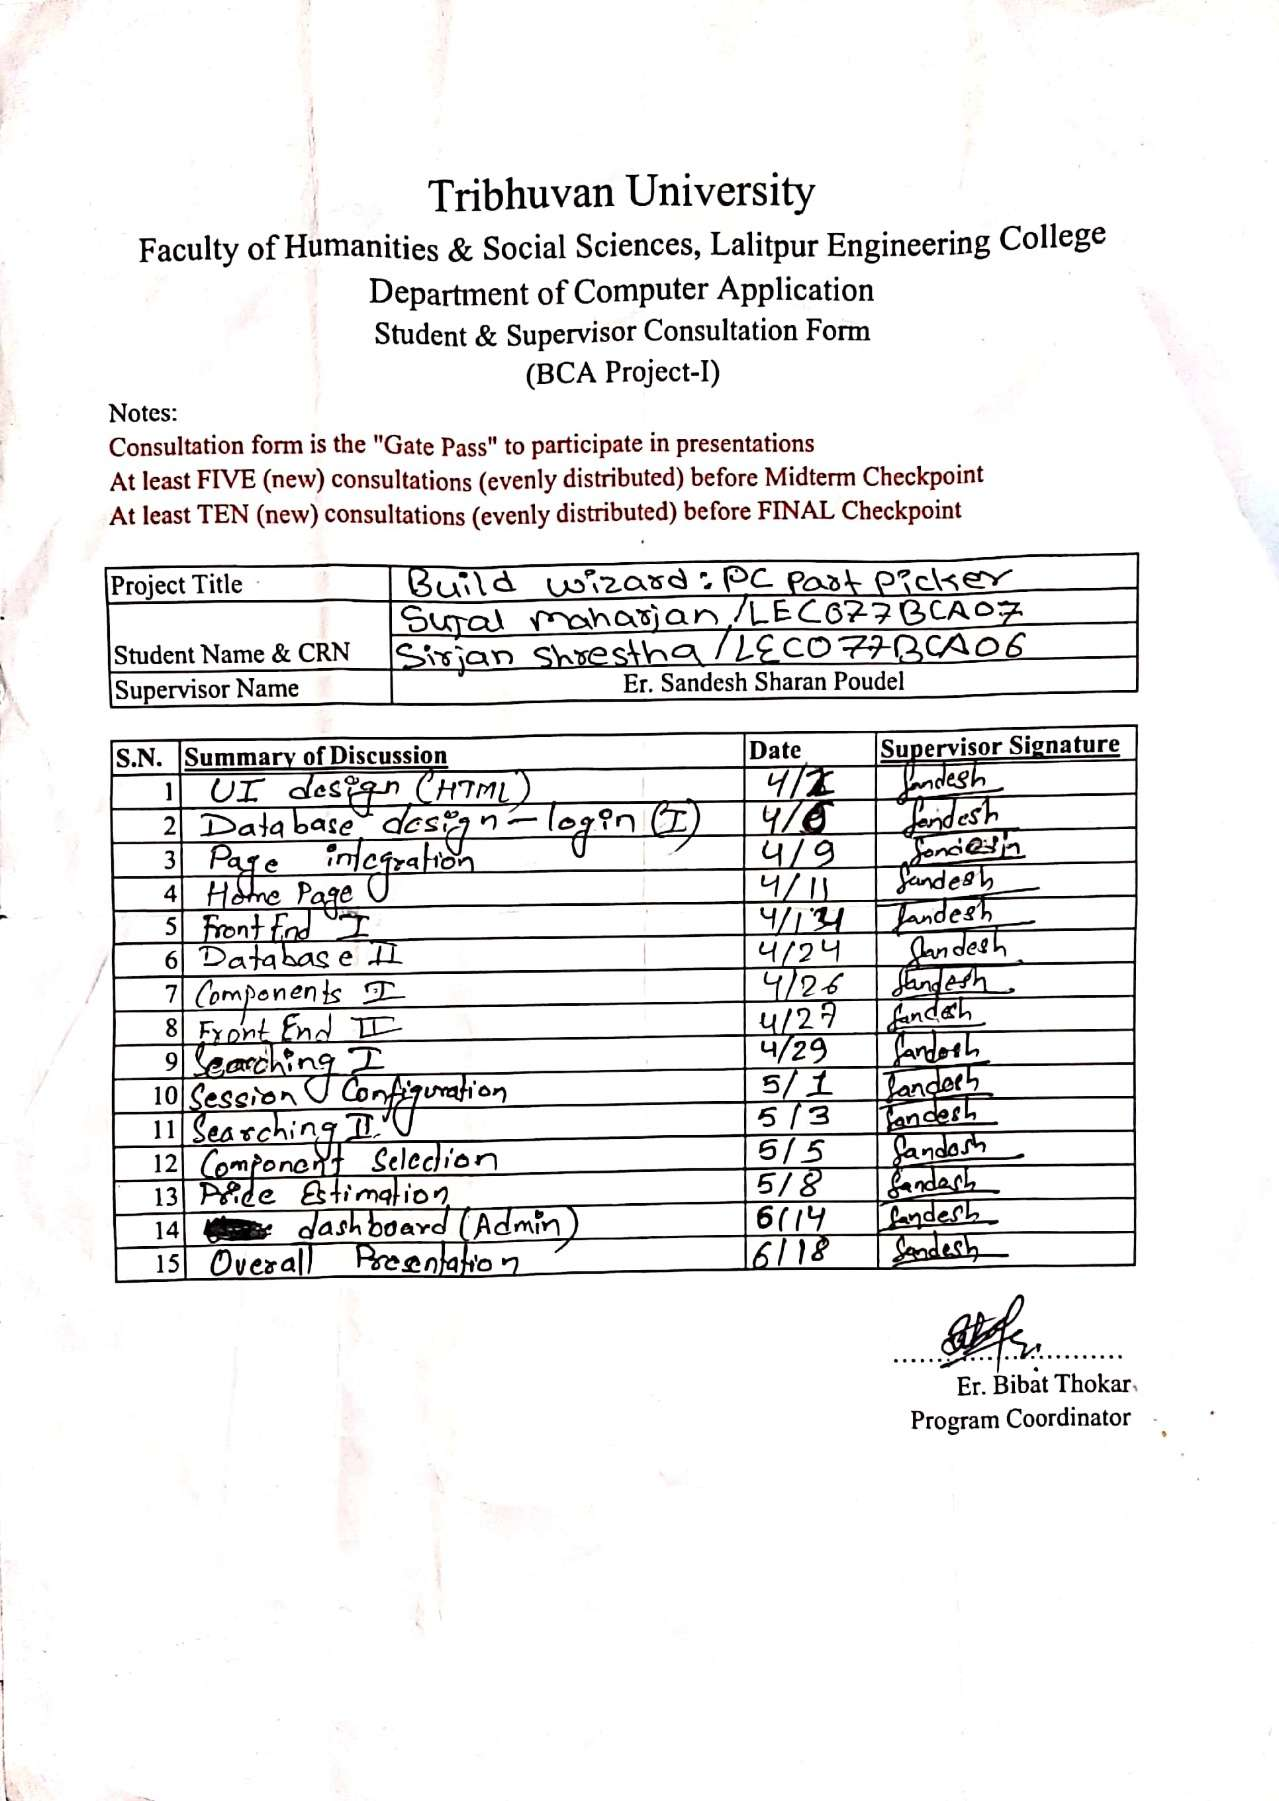
\includegraphics[width=400px]{Diagrams/supervisor.jpg}
\end{figure}



\input{Appendix/appendix2.tex}
\end{appendices}



%========================References setup=========================================================
\newpage
\bibliographystyle{unsrt}
\bibliography{References/references}

\addcontentsline{toc}{chapter}{REFERENCES}

%=============================================================================================



%=========================================================================
\end{document}